%===================================================================================
% JORNADA CIENTÍFICA ESTUDIANTIL - MATCOM,
%===================================================================================
% Esta plantilla ha sido diseñada para ser usada en los artículos de la
% Jornada Científica Estudiantil, MatCom.
%
% Por favor, siga las instrucciones de esta plantilla y rellene en las secciones
% correspondientes.
%
% NOTA: Necesitará el archivo 'jcematcom.sty' en la misma carpeta donde esté este
%       archivo para poder utilizar esta plantila.
%===================================================================================

%===================================================================================
% PREÁMBULO
%-----------------------------------------------------------------------------------
\documentclass[a4paper,10pt,twocolumn]{article}

%===================================================================================
% Paquetes
%-----------------------------------------------------------------------------------
\usepackage{amsmath}
\usepackage{amsfonts}
\usepackage{amssymb}
\usepackage{jcematcom}
\usepackage[utf8]{inputenc}
\usepackage{listings}
\usepackage[pdftex]{hyperref}
%\usepackage{stix}

\usepackage{graphicx}
\usepackage{caption}
\usepackage{subcaption}

\usepackage{algorithm}
\usepackage{algpseudocode}
\usepackage{amsmath}
\usepackage{verbatim}

%-----------------------------------------------------------------------------------
% Configuración
%-----------------------------------------------------------------------------------
\hypersetup{colorlinks,%
	    citecolor=black,%
	    filecolor=black,%
	    linkcolor=black,%
	    urlcolor=blue}
%===================================================================================

%===================================================================================
% Presentacion
%-----------------------------------------------------------------------------------
% Título
%-----------------------------------------------------------------------------------
\title{Influencia del Suavizado por Difusi\'on Anisotr\'opica (DA) en Im\'agenes de Ultrasonido.}

%-----------------------------------------------------------------------------------
% Autores
%-----------------------------------------------------------------------------------
\author{Ariel Plasencia D\'iaz\\
\name  \email \href{mailto:a.plasencia@estudiantes.matcom.uh.cu}{a.plasencia@estudiantes.matcom.uh.cu}
    \\ \addr C-412  \AND
Juan Carlos Esquivel Lamis \\
\name   \email \href{mailto:j.esquivel@estudiantes.matcom.uh.cu}{j.esquivel@estudiantes.matcom.uh.cu}
    \\ \addr C-411  \AND
Reinaldo Barrera Travieso\\
\name  \email \href{mailto:r.barrera@estudiantes.matcom.uh.cu}{r.barrera@estudiantes.matcom.uh.cu}
    \\ \addr C-411 }

%-----------------------------------------------------------------------------------
% Tutores
%-----------------------------------------------------------------------------------
\tutors{\\
Dra. Angela Le\'{o}n Mec\'ias, \emph{Universidad de La Habana} \\}

%-----------------------------------------------------------------------------------
% Headings
%-----------------------------------------------------------------------------------
\jcematcomheading{\the\year}{1-\pageref{end}}{Curso Optativo: Procesamiento de Im\'agenes Digitales}

%-----------------------------------------------------------------------------------
\ShortHeadings{}{Autores}
%===================================================================================

%===================================================================================
% DOCUMENTO
%-----------------------------------------------------------------------------------
\begin{document}

%-----------------------------------------------------------------------------------
% NO BORRAR ESTA LINEA!
%-----------------------------------------------------------------------------------
\twocolumn[
%-----------------------------------------------------------------------------------

\maketitle

%===================================================================================
% Resumen y Abstract
%-----------------------------------------------------------------------------------
\selectlanguage{spanish} % Para producir el documento en Español

%-----------------------------------------------------------------------------------
% Resumen en Español
%-----------------------------------------------------------------------------------
\begin{abstract}

En este trabajo se aplica el modelo de difusi\'on anisotr\'opica de Perona-Malik a un conjuntos de im\'agenes de ultrasonidos. Para este proceso primero se particiona la imagen empleando una t\'ecnica de segmentaci\'on de superp\'ixeles, en este caso $SLIC$("Simple Liner Iterative Clustering"). Una vez que son obtenidos estas regiones o segmentos se realiza un suavizado por regiones teniendo en cuenta la difusi\'on anisotr\'opica que a diferencia de la isotr\'opica, esta permite conservar los bordes. Tambi\'en se discute un nuevo algoritmo para aproximar lo que se conoce como par\'ametro de constraste $(k)$, el cual se emplea a la hora de obtener el coeficiente de difusi\'on.

\end{abstract}

%-----------------------------------------------------------------------------------
% English Abstract
%-----------------------------------------------------------------------------------
\vspace{0.5cm}
\begin{enabstract}
In this work, the Perona-Malik anisotropic diffusion model is applied to a set of ultrasound images. For this process, the image is first partitioned using a superpixel segmentation technique, in this case SLIC. Once these regions or segments are obtained, a region-wise smoothing is performed, taking into account the anisotropic diffusion that, inlike the isotropic, this allows to preserve the edges of the image. A new algorithm is also discussed to aproximate what is known as the contrast parameter, which is used to obtain the difussion coefficent.
\end{enabstract}

%-----------------------------------------------------------------------------------
% Palabras clave
%-----------------------------------------------------------------------------------
\begin{keywords}
Difusión anisotrópica, imágenes de borde, imágenes de ultrasonido, modelo de Perona-Malik, parámetro de contraste, difusión anisotrópica por regiones.
\end{keywords}

%-----------------------------------------------------------------------------------
% Temas
%-----------------------------------------------------------------------------------
\begin{topics}
An\'alisis de la detecci\'on de bordes en estas im\'agenes de ultrasonidos. Difusi\'on anisotr\'opica.
\end{topics}

%-----------------------------------------------------------------------------------
% NO BORRAR ESTAS LINEAS!
%-----------------------------------------------------------------------------------
\vspace{0.8cm}
]
%-----------------------------------------------------------------------------------

%===================================================================================
% Introducción
%-----------------------------------------------------------------------------------
\section{Introducción}\label{sec:introduccion}
%---------------------------------------------------------------
Las im\'agenes han estado presente a lo largo de la historia de la huminadad, pues ya desde que se conoce de la existencia del hombre, este se vio en la necesidad de dejar impregnada en las paredes de las cuevas, dibujos o im\'agenes de su vida diaria. Las im\'agenes se pueden ver como una figura o representaci\'on visual de objetos, ya sean reales o imaginarios, este vocablo proviene del lat\'in $imago$, que significa retrato. En este sentido puede tratarse de una pintura, un dibujo, un retrato, una fotograf\'ia o un video. Una imagen puede buscar representar la realidad, o sea, todo aquello que es visible por los ojos humanos, aunque tambi\'en puede tener una funci\'on simb\'olica. En t\'erminos de \'optica, estas se pueden ver como la reproducci\'on visual de la figura de un objeto captado a trav\'es de un lente que refleja o refracta los rayos de luz que de \'el proceden, ya sea reales o virtuales.

A lo largo del tiempo han existido una gran variedad de formas o tipos de im\'agenes, pero estas se ve\'ian afectadas por factores externos, ya sea por deterioro o elementos que degradaban la calidad de la misma. Con la entrada del mundo en la era digital, aparecen un nuevo tipo de im\'agenes, conocidas como im\'agenes digitales.

Una imagen digital es una representaci\'on bidimensional de una imagen a partir de una matriz n\'umerica, frecuentemente en binario. Estas se pueden obtener de varias formas, ya sea por alg\'un dispositivo de entrada haciendo una conversi\'on anal\'ogica digital como los esc\'aneres y c\'amaras digitales, o se pueden obtener a trav\'es de programas inform\'aticos de edici\'on de im\'agenes o dibujos de estas. Una de las tantas caracter\'isticas es que se pueden modificar mediantes filtros, a\~nadir o suprimir elementos, modificar su tama\~no y ser almacenadas en un dispositivo como discos duros o memorias. Con esta nueva modalidad de las im\'agenes surge una nueva rama de la computaci\'on, el procesamiento de im\'agenes digitales.

Pero, ?`qu\'e es el procesamiento de im\'agenes digitales? Este procesamiento no es m\'as que el conjunto de t\'ecnicas que se aplican a las im\'agenes digitales con el objetivo de mejorar la calidad o facilitar la obtenci\'on de informaci\'on. Este mecanismo es muy bien usado por la medicina hoy en d\'ia, ya que las im\'agenes digitales han tenido una gran repercusi\'on en varias ramas m\'edicas, dentro de estas podemos encontrar las mamograf\'ias, tomograf\'ias, rayos X, ultrasonidos, endoscop\'ias entre otras. En este campo no solo es de gran importancia la obtenci\'on de estas im\'agenes, sino que, con el procesamiento de im\'agenes, se recopila informaci\'on para estudios posteriores.

En el campo de mejoramiento de im\'agenes, los filtros juegan un importante papel, ya que este conjunto de t\'ecnicas tiene como objetivo fundamental obtener, a patir de una imagen original, otra final, cuyo resultado sea m\'as adecuado, mejorando ciertas caracter\'isticas de la misma que permiten realizar operaciones de procesado sobre ellas. Todo este proceso se realiza con el objetivo de suavizar la imagen, eliminar ruidos existentes y resaltar y detectar bordes. En lo general, los filtros se consideran como operaciones que se aplican a los p\'ixeles de una imagen digital para mejorarla, resaltar cierta informaci\'on o lograr efectos especiales en ella. A\'un siendo tan ventajoso la aplicaci\'on de filtros sobre una imagen nos encontramos con el percance de que el ruido no puede ser eliminado completamente, pero si llegar a un punto donde se permita extraer m\'as informaci\'on que en el estado original. 

En estad\'istica podemos encontrar la funci\'on gaussiana o campana de Gauss, la cual es una funci\'on definida por la expresi\'on

\begin{equation} \label{eqn:gauss}
	f(x) = ae^{-\frac{(x-b)^2}{2c^2}}
\end{equation}

Dicha funcio\'n presenta innumerables aplicaciones en el campo del procesamiento de im\'agenes digitales, ya que es utilizada como filtro de suavizado en las im\'agenes. Este filtro, similar al filtro de la media, provoca una disminuci\'on de la nitidez, aumento de la borrosidad y p\'erdida de detalles. 

A partir del filtro gaussiano se pueden obtener otras t\'ecnicas de filtrado, como la difusi\'on anisotr\'opica(DA) o tambi\'en llamada difusi\'on Perona-Malik. Esta es un t\'ecnica con el objetivo de reducir el ruido de una imagen sin afectar elementos importantes de la imagen, por lo general se estar\'ia hablando de los bordes, l\'ineas u otros detalles que son importantes para su interpretaci\'on. Este filtrado fue presentado por Pietro Perona y Jitendra Malik en julio de 1990 en un art\'iculo titulado "Scale-Space and edge detection using anisotropic Diffusion" \cite{perona_malik}. En su formulaci\'on original, el filtro de espacio-variante es, de hecho, is\'otropo, pero depende del contenido de la imagen, de forma que se aproxima a una funci\'on de impulso cerca de los bordes y otras estructuras que deben ser preservadas en la imagen sobre los diferentes niveles de escala resultante. Esta formulaci\'on se refiere a la difusi\'on anisotr\'opica por Perona y Malik aunque el filtro adaptado localmente es isotr\'opico, tambi\'en se ha referido a la difusi\'on como no homog\'eneo y no lineal.

Han sido varios los trabajos dedicados a este tema y en particular a este tipo de filtrado de difusi\'on anisotr\'opica y a\'un sigue siendo un tema para discutir en los d\'ias actuales. En la Tesis de Licenciatura en Matem\'atica "Difusi\'on anisotr\'opica aplicada a la detecci\'on de bordes en im\'agenes", defendida el 4 de julio del 2011 por el estudiante Mariano Rodr\'iguez Guerra, el cual aplic\'o este m\'etodo al suavizado de im\'agenes naturales e im\'agenes de la Aduana. Dos a\~nos despu\'es, en la Tesis de Maestr\'ia, "Estimaci\'on del par\'ametro de contraste en la ecuaci\'on de Perona-Malik", Michel Borroto Fern\'andez trabaja sobre la primera propuesta donde el coeficiente de difusi\'on cambia con el tiempo a trav\'es de la estimaci\'on en cada paso del umbral del gradiente, mediante un algoritmo de partici\'on y ajuste que llamamos $KMMC$.

Sin embargo, en el algoritmo $KMMC$ con im\'agenes de mamograf\'ia, se detect\'o un error en una de las cuentas (aunque esto no cambiaba el desempe\~no del algoritmo en im\'agenes naturales) y que para im\'agenes de mamograf\'ia muchas veces el algoritmo daba error ya que en la partici\'on K-medias la forma de calcular uno de los centroides, como la suma de los valores m\'aximo y m\'inimo del gradiente de intensidad, puede que sea un valor que no exista para estas im\'agenes, con lo cual se propuso una modificaci\'on al Algoritmo de Borroto, en la Tesis de Licenciatura en Ciencias de la Computaci\'on "Estimaci\'on del par\'ametro de contraste para el suavizado por difusi\'on anisotr\'opica aplicado por regiones.", de la estudiante Elizabeth Hidalgo-Gato Maim\'o \cite{hidalgo}, defendida en junio del 2015. Esta modicaci\'on fue nombrada $KMMC2$. En esta nueva versi\'on la difusi\'on se aplica por regiones, segmentando la imagen primero usando Superp\'ixels, $SLICS$, que es un algoritmo costoso computacionalmente. Por lo que en la Tesis de Licenciatura en Matem\'atica "Suavizado de im\'agenes por regiones: una versi\'on en paralelo con coeficiente variable en la difusi\'on anisotr\'opica", del estudiante Richard Miguel M\'endez Castillo, defendida 21 de junio del 2019, se propuso paralelizar el algoritmo $KMMC2$ y probar la efectividad de la difusi\'on en la preservaci\'on de los bordes para im\'agenes de mamograf\'ia \cite{richard}.

Dado que los algoritmos de procesamiento de im\'agenes no son universales y no tienen el mismo desepe\~no para todo tipo de im\'agenes, se propone en este trabajo probar el algoritmo desarollado por Richard en 2019 para el suavizado de im\'agenes de Ultrasonido y analizar su influencia en la posterior detecci\'on de bordes en este tipo de im\'agenes. En la secci\'on 1 se presentar\'a el proceso de difusi\'on en im\'agenes y la teor\'ia b\'asica de modelos matem\'aticos para la compresi\'on sobre este tipo de filtrado. La secci\'on 2 explicar\'a el algoritmo $KMMC$ y $KMMC2$ junto con las t\'ecnicas utilizadas por estos. En la secci\'on 3 se pasar\'a a la parte experimental del trabajo, donde se aplicar\'a el algoritmo a las im\'agenes de Ultrasonido analizando los resultados obtenidos.
%===================================================================================

\subsection{Difusi\'on de im\'agenes}\label{sec:difusion_imagenes}

La difusi\'on es la acci\'on y efecto de difundir y entre sus sin\'onimos podemos encontrar propagar, divulgar y esparcir. La difusi\'on f\'isica est\'a sujeta a la Ley de Fick, que sostiene que la membrana permeable permite el paso de part\'iculas y disolvente a favor del gradiente de concentraci\'on. La primera ley de Fick para una \'unica dimensi\'on toma la forma:

\begin{equation}
	J = -D \frac{\partial \phi}{\partial x}
\end{equation}
donde $J$ es el flujo difusivo, $D$ es el coeficiente de difusi\'on, $\phi$ la concentraci\'on y por \'ultimo $x$ es la posici\'on dado en posici\'on de longitud. Para dos o m\'as dimensiones, podemos hacer uso del operador $\nabla$ (nabla o gradiente), lo cual generaliza la primera derivada, obteni\'endose:

\begin{equation}
	J = -D \nabla \phi
\end{equation}

Para este trabajo utilizaremos otra notaci\'on para esta f\'ormula qued\'andonos de la forma:

\begin{equation}
	j = -c \cdot \nabla I
\end{equation}
donde $c$ es el coeficiente de difusi\'on y $\nabla I$ el gradiente de concentraci\'on.

Como la difusi\'on solo es un procesos que transporta masa sin destruirla, ni crear nueva, se cumple la ley de conservaci\'on y de forma matem\'atica se expresa mediante la ecuaci\'on de continuidad, donde $t$ denota el tiempo:

\begin{equation}
	\frac{\partial I}{\partial t} = - div j
\end{equation}
siendo $div$ el operador de divergencia. Si se sutituye la primera ley de Fick en esta ecuaci\'on de continuidad terminamos teniendo la siguiente ecuaci\'on de difusi\'on:

\begin{equation}
	\frac{\partial I}{\partial t} = div(c \cdot \nabla I)
\end{equation}

Pero como este concepto se desea adaptar a una imagen en escala de grises, la cual se representa mediante una funci\'on $u:\Omega \subset \mathbb{R}^2 \rightarrow G \subset \mathbb{Z}$ donde G = [0, 255] (0 es negro y 255 es blanco) representa los niveles de grises en la posici\'on $(x,y)$. Para esto tomamos la funci\'on $I: \mathbb{R}^3 \rightarrow G \subset \mathbb{Z}$ donde $I(x,y,t) = \{u(x,y)\ |\ en\ el\ momento\ t\ de\ la\ imagen\}$ y teniendo que $c$ es el coeficiente de difusi\'on se puede rescribir la \'ultima ecuaci\'on como:

$$
\begin{cases}
\frac{\partial I}{\partial t} = div(c(x,y,t) \cdot \nabla I(x,y,t)) \\
I(x,y,0) = I_0
\end{cases}  
(1)
$$

En este caso la difusi\'on pertenece a un espacio multiescala, donde su idea principal es que a partir de una imagen inicial $I_0$, se genera una familia $I(x,y,t)$, donde se van obteniendo versiones de im\'agenes gradualmente m\'as suaves seg\'un se va aumentando la escala, en este caso el tiempo $t$.

En el procesamiento de im\'agenes podemos identifiacar la concentraci\'on con los valores de grises en una cierta ubicaci\'on de la imagen. Si el coeficiente de difusi\'on es constante en todo el dominio de la imagen, se habla de difusi\'on homog\'enea o isotr\'opica. Isotrop\'ia en la difusi\'on de im\'agenes se interpreta como que cada p\'ixel se trata de la misma manera, independientemente de sus caracter\'isticas como el gradiente. Esto trae algunos incovenientes como por ejemplo, el uso de suavizado gaussiano \cite{galic}, no solo reduce el ruido sino tambi\'en difumina caracter\'isticas importantes como los bordes y, por tanto, hace que sean m\'as dif\'iciles de identificar, adem\'as de no respetar el borde natural de los objetos.

Dado a las limitaciones y p\'erdida de informaci\'on con la difusi\'on isotr\'opica, Perona y Malik dise\~naron un algoritmo en \cite{perona_malik} que elimina el ruido mientras conserva las carectir\'isticas de los bordes. Los autores proponen para hacer el suavizado dentro de la regi\'on de cada imagen, delimitado por bordes y no alise estos bordes. Por tanto tenemos tres principos que tiene que cumplir esta nueva difusi\'on:

\begin{enumerate} 
\item {Causalidad: Cualquier caracter\'istica con un nivel de resoluci\'on aproximado debe poseer una causa (no necesariamente \'unica) en un nivel m\'as fino de resolución, aunque lo contrario no tiene por qu\'e ser cierto. En otras palabras, ning\'un detalle espurio debe ser generado cuando la resoluci\'on es disminuida.}
\item {Localizaci\'on inmediata: En cada resoluci\'on, los l\'imites de la regi\'on deben ser n\'itidas y coincidir con los l\'imites sem\'anticamente significativos en esa resoluci\'on.}
\item {Suavizado por partes: En todas las escalas, debe producirse un suavizado intrarregional preferentemente sobre el suavizado entre regiones. Esto significar\'ia que los c\'irculos se suavizar\'an primero en el interior, y no a trav\'es de la circunferencia.}
\end{enumerate}

%-----------------------------------------------------------------------------------
\subsection{El operador gradiante discreto}\label{sec:operador_gradiente}

Como ya se mencion\'o anteriormente una imagen se representa mediante una funci\'on bidimensional que describe la intensidad en cada p\'ixel. Los p\'ixeles de bordes los podemos identificar donde ocurren cambios bruscos en el nivel de gris, o sea, donde ocurre una mayor variaci\'on en la intensidad. Esto lo podemos ver como el operador del gradiante $||\nabla I||$.

Ya sabemos que la funci\'on de una imagen digital retorna valores enteros y en el caso de las de escala de grises, estos valores precisamente se encuentran entre el intervalo $\left[ 0, 255 \right] $, por lo tanto el conjunto imagen de esta funci\'on es un conjunto discreto, esto implica que el operador gradiente a usar se deriva del continuo conocido, por lo que se necesita una buena aproximaci\'on de su forma discreta.

En el caso que se asuma la diferenciabilidad de la funci\'on $I(x,y)$ y utilizando diferenciales, tenemos que:

\begin{equation}
	I(X + \vec{h}) - I(X) \approx \frac{\partial I}{\partial x}h_1 + \frac{\partial I}{\partial y}h_2
\end{equation}
donde $\vec{h} =\left ( \begin{array}{c} h_1 \\ h_2 \end{array} \right )$ representa el vector incremento y $X = (x_0, y_0)$.

Si se desea aproximar $\frac{\partial I}{\partial x}$ en el punto $X = (x,y)$, podemos ultilizar:

\begin{equation}
	\left [ \begin{array}{ccc} 
		I(x-1, y-1) & I(x, y-1) & I(x+1, y-1) \\
		I(x-1, y)   & I(x, y)   & I(x+1, y) \\
		I(x-1, y+1) & I(x, y+1) & I(x+1, y+1) 
	\end{array} \right ]
\end{equation}

Usando esta opci\'on de aproximaci\'on por diferencias espaciales, podemos estimar el gradiente mediante cuatro componentes direccionales, las cuales indican los los puntos cardianles:

\begin{equation}
	\nabla_N(I(x,y)) = I(x,y-1) - I(x,y)	
\end{equation}

\begin{equation}
	\nabla_S(I(x,y)) = I(x,y+1) - I(x,y)	
\end{equation}

\begin{equation}
	\nabla_E(I(x,y)) = I(x-1,y) - I(x,y)	
\end{equation}

\begin{equation}
	\nabla_W(I(x,y)) = I(x+1,y) - I(x,y)	
\end{equation}

Para este trabajo usaremos la siguiente expresi\'on teniendo en cuenta la diferencia hacia adelante:

\begin{equation}
	\frac{\partial I}{\partial t} = I(x, y, t+1) - I(x,y,t)
\end{equation}

Teniendo en cuenta todas estas expresiones se puede obtener la siguiente aproximaci\'on: \\

$I_{x,y,t+1} \approx \lambda (cN_{x,y,t} \nabla N(I_{x,y,t}) + cS_{x,y,t} \nabla S(I_{x,y,t}) + cE_{x,y,t} \nabla E(I_{x,y,t}) + cW_{x,y,t} \nabla W(I_{x,y,t})) + I_{x,y,t}$ \\

donde $cN_{x,y,t},\ ... \, cW_{x,y,t}$ se refieren a los valores del coeficiente de difusi\'on para los gradiantes seg\'un su componente direccional. Para esto tomamos $0 < \lambda < \frac{1}{4}$ para mantener la estabilidad num\'erica del esquema de soluci\'on.

%-----------------------------------------------------------------------------------
\subsection{El coeficiente de difusi\'on}\label{sec:coeficiente_difusion}
		
Una de las limitantes de la difusi\'on isotr\'opica es que este filtrado ocurre en todo los p\'ixeles de la imagen, incluyendo los bordes. El causante de este problema es $c$, el coeficente de difusi\'on que en este caso se toma de forma constante, por lo que se le aplica la misma difusi\'on a todos los p\'ixeles de la imagen. La idea en el caso de la difusi\'on anisotr\'opica es sustituir este coeficiente por una funci\'on de tal forma que se logre una variaci\'on del mismo en diferentes puntos de la imagen y a\'un siga cumpliendo con los principios planteados con anterioridad.

Para lograr la preservaci\'on de los bordes, debemos encontrar una funci\'on para el coeficiente que impida o que se haga de forma m\'as leve la difuminaci\'on cuando estemos en presencia de un borde, mientras que en el caso contrario buscamos que esta difuminaci\'on sea mucho mayor. La selecci\'on de tal funci\'on es de suma importancia en la difusi\'on anisotr\'opica. 

Intuitivamente se pudiera pensar en la siguiente funci\'on para el coeficiente:

$$
C(x,y,t)=
\begin{cases}
c(x,y,t) = 0 & el\ pixel\ (x,y)\ es\ borde \\
c(x,y,t) = 1 & en\ otro\ caso 
\end{cases}
$$

En este caso la funci\'on $C$ solo aplicaria la difusi\'on a los p\'ixeles que no sean bordes, ya que de serlo toda la expresi\'on ser\'ia cero. De esta manera el suavizado se lograr\'a con el tercer principio expuesto por Perona y Malik \cite{perona_malik}.

Una vez conocido que $||\nabla I||$ es la variaci\'on de intensidad en escala de gris de cada p\'ixel y que cuando los valores de esta cambian de forma repentina es que estamos en precencia de un borde de la imagen. Para esto, necesitamos una funci\'on de la forma $c(x,y,t) = g(|| \nabla I(x,y,t) ||)$ que cumpla con los siguientes requisitos:

\begin{enumerate} 
\item $g(x)$ mon\'otona decreciente.
\item $\lim_{x \to 0}\ g(x) = 1$
\item $\lim_{x \to \infty}\ g(x) = 0$
\end{enumerate}

La condici\'on 1 garantiza el suvizado isotr\'opico en regiones de semejante intensidad, mientras que las condiciones restantes permiten mantener los bordes visibles. Existen varias expresiones para la funci\'on de difusi\'on $g$, algunas de estas pueden ser consultadas en \cite{borroto}. Para el desarrollo de este trabajo y dando continuidad a los temas antecesores por los cuales este se rige se seleccion\'o entre varias propuestas de Perona y Malik \cite{perona_malik}, la expresi\'on $g_2(s) = exp(\frac{-s^2}{k^2})$ y haciendo la sustituci\'on $s=||\nabla I||$ el coeficiente de difusi\'on queda de la siguiente forma:

\begin{equation}
	c(x,y,t) = e^{-(\frac{||\nabla I(x,y,t)||}{k})^2}
\end{equation}

Esta funci\'on cumple con los tres requsitos planteados anteriormente, pues ya tenemos una funci\'on para el coeficiente de difusi\'on, pero a\'un tenemos que encontrar al par\'ametro $k$. En (14) se muestra que en esos lugares de la imagen donde $|| \nabla I || > k$ son considerados como bordes, por lo que el proceso de difusi\'on tiene un menor efecto, por lo tanto, los bordes son preservados y en el caso contrario el coeficiente se incrementa ocurriendo una mayor difuminaci\'on puesto que se trata de regiones que no pertenecen a los bordes, por lo que $k$ es un par\'ametro de contraste o umbral del gradiente. 

%===================================================================================
% Desarrollo
%-----------------------------------------------------------------------------------
\section{Desarrollo}\label{sec:desarrollo}
%-----------------------------------------------------------------------------------

En la secci\'on anterior se analiz\'o y busc\'o una expresi\'on para el coeficiente de difusi\'on que permitiera la conservaci\'on de los bordes y el suavizado fuera de estos. Por \'ultimo se observ\'o la importancia de seleccionar un valor para el par\'ametro de contraste, el cual permita que el coeficiente de difusi\'on logre una difusi\'on anisotr\'opica. 

%-----------------------------------------------------------------------------------
\subsection{M\'etodo de partici\'on y ajuste ($KMMC$)}\label{sec:kmmc}

El m\'etodo de partici\'on y ajuste presentado en \cite{borroto}	se desarrolla utilizando un algoritmo de agrupaci\'on K-Means con $K=3$. Sea $P$ el conjunto de todos los p\'ixeles de la imagen, la idea es dividir este grupo en tres conjuntos disjuntos $P_1,\ P_2\ y\ P_3$. A trav\'es de un ajuste de la curva de m\'inimos cudrados definida por el coeficiente de difusi\'on dado en (10) se selecciona los puntos utilizados para aproximar los par\'ametros de contraste $k$.

K-means es un m\'etodo de agrupamiento, que tiene como objetivo la partici\'on de un conjunto de n observaciones en $m$ grupos en el que cada observaci\'on pertenece al grupo cuyo valor medio es m\'as cercano. Dado un conjunto de observaciones $\{x_1, x_2, …, x_n\}$, $K-Means$ construye una partici\'on de las observaciones en $m$ conjuntos $S = \{S_1, S_2, …, S_m\}$ donde $(m \leq n)$ a fin de minimizar la suma de los cuadrados dentro de cada grupo.

\begin{equation}
	min \sum_{i=1}^m \sum_{x_j \in S_i} d(x_j, u_i)^2
\end{equation}
donde $u_i$ es la media o centroide de $S_i$ y $d(x, y)$ es la distancia entre dos objetos.

La idea b\'asica de K-Means puede ser implementada de la siguiente forma:

\begin{enumerate} 
\item {Seleccionar $m$ medias o centroides iniciales.}
\item {Cada elemento es asignado al grupo con el centroide m\'as cercano.}
\item {Los centroides son recalculados.}
\item {Repetir desde el paso 2 hasta que se alcance alg\'un criterio de parada, como limitar las iteracciones o cuando ning\'un objeto cambie de grupo.}
\end{enumerate}

Al aplicar este algoritmo se van a repartir los p\'ixeles en $P$ bajo los siguientes criterios:

\begin{itemize} 
\item $P_1$: Subconjunto de p\'ixeles que no pertenecen a los bordes de la imagen(menor gradiente). 
\item $P_3$: Subconjunto de p\'ixeles que si pertenecen a los bordes de la imagen(mayor gradiente).
\item $P_2 = P - (P_1 \cup P_3)$: Subconjunto de p\'ixeles que no se conoce con seguridad si pertencen o no a los bordes de la imagen. 
\end{itemize}

Por tanto, como par\'ametros del algoritmo K-Means se tiene que:

\begin{itemize} 
\item {N\'umero de grupos:
	\begin{equation}
		K = 3
	\end{equation}}
\item {Medias o centroides iniciales:
	\begin{equation}
		\mu_1 = min \{||\nabla I||_{(x,y)} : (x,y) \in P\}\ para\ P_1
	\end{equation}
	\begin{equation}
		\mu_2 = \frac{\mu_1 + \mu_3}{2}\ para\ P_2
	\end{equation}
	\begin{equation}
		\mu_3 = max \{||\nabla I||_{(x,y)} : (x,y) \in P\}\ para\ P_3
	\end{equation}}
\item {Operaciones: \\
	\begin{itemize} 
		\item {Distancia: 
			\begin{equation}
				d((x,y), \mu_i) = \left| \parallel \nabla I \parallel_{(x,y)} - \mu_i \right|\  i=1,2,3
			\end{equation}}
		\item {Suma:
			\begin{equation}
				a((x_1,y_1), (x_2,y_2)) = ||\nabla I||_{(x_1,y_1)} + ||\nabla I||_{(x_2,y_2)}
			\end{equation}}
	\end{itemize}}
\end{itemize}

Sean $p_2$ y $p_3$ los menores valores en magnitud del gradiente de los p\'ixeles pertenecientes a los subconjuntos $P_2$ y $P_3$  respectivamente. Para controlar la intensidad del difuminado se definen dos umbrales $upbd(wep)$ como preservaci\'on de bordes d\'ebiles y $upbf(sep)$, de preservaci\'on de bordes fuertes. Estos valores son en verdad los valores del coeficiente de difusi\'on que se quieran hacer corresponder a los valores del gradiente de intensidad $p_2$ y $p_3$.

Los p\'ixeles de $P_3$ que son de bordes fuertes se difuminan con intensidad menor que $sep$ y los de bordes d\'ebiles se difuminan con intensidad menor que $wep$, por consiguiente el umbral $sep$ debe tomarse cercano a 0 mientras que $wep$ debe tomar informaci\'on de la imagen.

Una vez que se tenga los puntos $(p_2,\ sep)$ y $(p_3,\ wep)$ el par\'ametro de constraste $k$ ser\'a obtenida mediante una aproximaci\'on m\'inima cuadr\'atica de la funci\'on (2), entonces se define la funci\'on $S$ de la forma:

\begin{equation}
	S(k) = \left [sep - e^{-(\frac{p_2^2}{k^2})^2} \right ]^2 + \left [wep - e^{-(\frac{p_3^2}{k^2})^2} \right ]^2
\end{equation}
y resolviendo la ecuaci\'on:

\begin{equation}
	\frac{\partial S}{\partial k} = 0
\end{equation}

Finalmente, obtenemos la siguiente expresi\'on para el par\'ametro de contraste $k$:

\begin{equation}
	k = \sqrt{- \frac{p_2^2 + p_3^2}{\ln{(sep \times wep)} }}
\end{equation}

El algoritmo $KMMC$ nos muestra el proceso de particionamiento seg\'un K- Means, donde es evidente la existencia de valores menores (17) y mayores (19) del gradiente de intensidad de las im\'agenes. Visualicemos lo que est\'a sucediendo: como un recurso, podemos pensar que en cualquier matriz num\'erica se puede encontrar el m\'aximo y el valor m\'inimo; pero tambi\'en puede encontrar valores mayores que el m\'inimo y valores inferiores al m\'aximo. Estos valores intermedios est\'an representadosen el algoritmo KMLS, como la media de los dos valores extremos (18).

Luego, buscando valores medios de intensidad del gradiente, para hacer un d\'ebil suavizado de esos p\'ixeles. Pero esos valores no tienen por qu\'e existir o estar dentro del rango num\'erico de valores de instensidad asignados a la imagen. Esto podr\'ia conducir a una situaci\'on problem\'atica cuando el grupo, cuyo centroide es (18), permanece vac\'io.

Por lo general, las im\'agenes tienen suficiente contraste y hay mucha variaci\'on en las intensidades de los p\'ixeles, pero en este trabajo, la imagen a la que se aplicar\'a el algoritmo va a ser un segmento. Entonces puede suceder que el segmento posea una caracter\'istica interesante, que cada p\'ixel tiene valores de gradiente similares, ya sea porque el segmento es un borde de la misma zona y los valores son iguales y positivo, o porque esta regi\'on es completamente del mismo color y el degradado es cero.

El problema del bajo contraste llev\'o a la idea de introducir la segmentaci\'on de la imagen antes de ejecutar cualquier proceso de difusi\'on, intentando suavizar localmente la imagen, para reforzar los bordes d\'ebiles.

%-----------------------------------------------------------------------------------
\subsection{Superp\'ixel}\label{sec:superpixel}

Un superp\'ixel puede ser definido como un grupo de p\'ixeles que comparten ciertas caracter\'isticas como por ejemplo la intensidad en escala de gris. Este est\'a comenzando a ser de gran utilidad en muchos algoritmo de Visi\'on por Computadora y Procesamineto de im\'agenes como son la segmentaci\'on de im\'agenes, etiquetado sem\'antico, detecci\'on de objetos y seguimiento. Esta t\'ecnica reduce la complejidad  de procesar las subsecuencias de una imagen, haci\'endolo de manera m\'as \'agil \cite{darshita}.

La t\'ecnica de superp\'ixeles se puede dividir en dos enfoques \cite{mark}:

\begin{itemize} 
	\item M\'etodos basados en grafos 
	\item M\'etodos de agrupamiento o crecimiento de regiones (ascenso del gradiante).
\end{itemize}

Lamentablemente no todas los enfoques de superp\'ixeles llevan estas especificaciones, como se muestra en \cite{achanta}. Por esto en este trabajo se propuso el uso del conocido algoritmo $SLIC$.
%-----------------------------------------------------------------------------------
\subsection{Simple Liner Iterative Clustering (SLIC)}\label{sec:slic}

Quiz\'as uno de los m\'etodos de superp\'ixeles m\'as usado es la t\'ecnica de $SLIC$ presentado en \cite{perona_malik}. Esta t\'ecnica genera regiones de im\'agenes significativas, utilizando agrupaci\'on para crear un superp\'ixel de tama\~no uniformemente compacto que describe adecuadamente la estructura de los objetos en una imagen \cite{mark}.

$SLIC$ adpata el m\'etodo de agrupamiento de K-Means visto anteriormente para generar de una forma eficiente los superp\'ixeles de la imagen. Por defecto es asumible que solo depende de un par\'ametro, el mismo que su algoritmo base K-Means el $k$ que define la cantidad de superp\'ixeles aproximadamente de igual tama\~no en que se desea particionar la imagen.

En esta t\'ecnica cada p\'ixel se caracteriza por un vector de 5 dimensiones, donde tres componentes representan el color y las dos restantes la posici\'on. Sin embargo, el procesamiento en el algoritmo es muy general y puede obtener resultados plausibles mediante el uso de medias alternativas de similitud, por lo que tambi\'en puede acomodar im\'agenes en escala de grises \cite{mark}. La similitud entre p\'ixeles se define como:

\begin{equation}
	D = d_c + m\frac{d_s}{s}
\end{equation}
donde $d_c$ y $d_s$ son el color y la diferencia espaciales respectivamente. Dados dos puntos (p\'ixeles $p_i$ y $p_j$) con cordenadas $(x_i, y_i)$ y $(x_j, y_j)$ y componentes de color $(l_i, a_i, b_i)$ y $(l_j, a_j, b_j)$ tenemos que:

\begin{equation}
	d_s(p_i, p_j) = \sqrt{(x_j - x_i)^2 + (y_j - y_i)^2}
\end{equation}

\begin{equation}
	d_c(p_i, p_j) = \sqrt{(l_j - l_i)^2 + (a_j - a_i)^2 + (b_j - b_i)^2}
\end{equation}

Dado a que en este trabajo solo se trabaja con im\'agenes de escala de grises las componentes del color en este caso ser\'ia de una sola dimensi\'on, la cual no indica la intensidad en dicho p\'ixel, entonces $d_c$ nos quedar\'ia de la forma:

\begin{equation}
	d_c(p_i, p_j) = \sqrt{(l_j - l_i)^2}
\end{equation}

Para determinar la pertenencia a un grupo y en lo sucesivo en este trabajo se define como la m\'etrica de dos p\'ixeles de la siguiente forma:

\begin{equation}
	D = \sqrt{\left (\frac{d_s}{N_s} \right )^2 + \left (\frac{d_c}{N_c} \right )^2}
\end{equation}

Con el objetivo de lograr la consistencia de los segmentos, se define $N_s$ con la mayor distancia espacial y $N_c$ como la mayor diferencia de color, con la idea de normalizar la medida D, ver en \cite{achanta}.

El orden de complejidad de este algoritmo es $O(N)$, mientras que K-Means es $O(kNi)$ done $N$ es el n\'umero de p\'ixeles de la imagen, $i$ el n\'umero de iteraciones y $k$ la cantidad de grupos en que se particiona. Esto se debe a que $SLIC$, limita el espacio de b\'usqueda de cada grupo a regiones de $2S \times 2S$ alrededor del p\'ixel central, donde $s = \sqrt{\frac{N}{k}}$; lo que hace que el tama\~no de cada superp\'ixel sea cercano a $S \times S$ y que la complejidad del algoritmo no dependa del número de superp\'ixeles o grupos $k$.

En lo adelante en cada ocasi\'on que se haga alusi\'on a regi\'on, segmento, subimagen o superp\'ixel; enti\'endase que son obtenidas a trav\'es de la t\'ecnica reci\'en explicada SLIC sobre la imagen original que se desea procesar.
%-----------------------------------------------------------------------------------
\subsection{KMMC2: nueva versi\'on del algoritmo KMMC}\label{sec:kmmc2}

Teniendo en cuenta los detalles negativos detectados en $KMMC$, se propuso algunas modificaciones:

\begin{enumerate} 
\item Para evitar que en ciertos momentos el grupo $P_2$ se quede vac\'io, K-Means se ejecuta para $K=2$. Denotando estos dos grupos como $G_1$ y $G_2$, en donde est\'an agrupado inicialmente por el m\'inimo (12a) y el m\'aximo (12b) respectivamente.
\item Otro cambio ser\'ia el de seleccionar de estas particiones el valor del gradiente utilizado posteriormente. Siguiendo el convenio tenemos que:

\begin{itemize} 
\item $p'_2$ como el valor de la media o centroide final de K-Means para el conjunto $G_1$. 
\item $p'_3$ como el valor de la media o centroide final de K-Means para el conjunto $G_2$. 
\end{itemize}

Sabiendo que los centroides representan el valor promedio de los elementos de un grupo, se  puede establecer una analog\'ia entre el KMMC original y esta versi\'on: Se crean tres grupos como en KMMC $(P'_1 \approx P_1, P'_2 \approx P_2, P'_3 \approx P_3)$, a partir de $G_1$ y $G_2$ de la forma siguiente:

\begin{equation}
	P'_1 = \{x \in G_1 : x < p'_2 \}
\end{equation}

\begin{equation}
P'_2 = \{x \in (G_1 \cup G_2) : p'_2 < x < p'_3 \}
\end{equation}

\begin{equation}
	P'_3 = \{x \in G_2 : x > p'_3 \}
\end{equation}

Esta \'ultima muestra los valores intermedios buscados en KMMC. Ya con esta conversi\'on de la versi\'on antigua a la nueva, podemos continuar en el algoritmo original.
Si hacemos $p_2 = p'_2$  donde $p'_2$ es el menor valor del conjunto $P'_2$ y $p_3 = p'_3$ ya que $p'_3$ es tambi\'en el menor valor del grupo $P'_3$. Por tanto es posible concluir de que el nuevo algoritmo toma como valores de variaci\'on de intensidad para ajustar la funci\'on a las medias o centroides de los grupos que en el mismo se define.

\item  Como los segmentos pueden ser im\'agenes con poco contraste, los valores de variaci\'on de intensidad de sus p\'ixeles son casi id\'enticos, sucede que los centroides iniciales son iguales, por tanto no tiene sentido efectuar el proceso K-Means, dado que el grupo es el mismo conjunto de variaci\'on de intensidad de toda la subimagen. En este caso solamente se realizar\'a la fase de ajuste con un \'unico punto, cuya coordenada de intensidad ser\'a $p'_0 = (2,1) = (2,2)$.

Solo nos restar\'ia saber los valores alcanzados por (10) para $p'_0$. Para esto se utiliza una estrategia basada en una an\'alisis global de los valores extremos de variaci\'on de intensidad.

\begin{itemize} 
\item Este algoritmo fue pensado inicialmente para ser aplicado a una imagen que es un segmento o parte de otra imagen de mayor tama\~no, haciendo que todo el an\'alisis realizado sea un proceso local. Tomando $G_{max}$ y $G_{min}$ como la mayor y la menor variaci\'on de intensidad de la imagen completa respectivamente. Entonces se podr\'a saber si $p'_0$ est\'a en el rango de intensidad alto o de borde si:

\begin{equation}
	G_{max} - p'_0 < G_{min} - p'_0
\end{equation}
en este caso, est\'a m\'as cerca del mayor valor, por tanto, para aproximar (2) se utiliza el valor $sep$ para alcanzar una difuminaci\'on d\'ebil. Por otra parte si se tiene que:

\begin{equation}
	G_{max} - p'_0 > G_{min} - p'_0
\end{equation}
pasa lo contrario, este se encuentra m\'as cerca del menor valor, empleando el $wep$ para lograr un alto difuminado. Dado esto ya podemos ajustar (17) con $n=1$ quedando:

\begin{equation}
	k = \sqrt{\frac{-x_1^2}{\ln {f(x_1)}}}
\end{equation}

Sustituyendo $x_1 = p'_0$ y $f(x_1) = {wep,\ sep}$ en dependencia a (33) y (34).

\item En (35) se cumple que en el caso que $p'_0 = 0$ entonces $k=0$ lo que indefine a (10), pero como $p'_0=0$ entonces la funci\'on $c(x,y,t)=1$ y no es necesario que se ajuste la curva. Esta situaci\'on es similar a una difusi\'on isotr\'opica en una imagen homog\'enea (sin contraste ni bordes), lo cual no es problema ya que no existen caracter\'isticas que conservar.
\end{itemize}

\end{enumerate}

%-----------------------------------------------------------------------------------
\subsection{Ajuste local vs Ajuste global}\label{sec:ajuste_local_ajuste_global}

Sabiendo de la existencia de regiones de bajo constraste y el funcionamiento del algoritmo de partici\'on global (imagen completa) y local (por regiones) expuestos anteriormente posibilita llegar a la siguiente observaci\'on:

Sea $I_0$ la imagen original y $I_{0_s}$ un segmento o regi\'on de $I_0$ de m\'inimo contraste, es decir que el nivel de gradiente de $I_{0_s}$ diferente de 0 se encuentra en una vencidad de cero, denotado por $P_{min}$.

\begin{itemize}
\item ?`Qu\'e pasa en el KMMC global?

$P_{min}$ pertenece al conjunto de los menores valores de gradiente de la imagen. Por tanto, los valores del coeficiente de difusi\'on (10) asociado con $P_{min}$ estar\'a cerca de 1, lo que implica que estar\'an fuertemente suavizado y se perder\'a el borde d\'ebil, mezcl\'andolo como en una difusi\'on isotr\'opica.

\item ?`Qu\'e pasa en el KMMC local?

Observando que en la regi\'on $I_{0_s}$, los elementos de $P_{min}$ podr\'ian pertenecer al conjunto de los mayores valores de variaci\'on de intensidad del segmento, ocurre que el valor de su coeficiente de difusi\'on asociado, es ajustado con $sep$, por tanto es un valor cercano a 0. Con esto se logra tratar al conjunto $P_{min}$ como p\'ixeles de bordes, siendo intensificados o no modificados.
\end{itemize}

En el resto de los casos ocurre de manera similar pero siempre aprovechando la mayor cantidad de informaci\'on de la imagen que brinda la difusi\'on local.
%----------------------------------------------------------------------------
\subsection{Algortimo DA-KMMC2}\label{sec:algoritmo_da_kmmc2}

\begin{figure}[htb]
	\begin{center}
		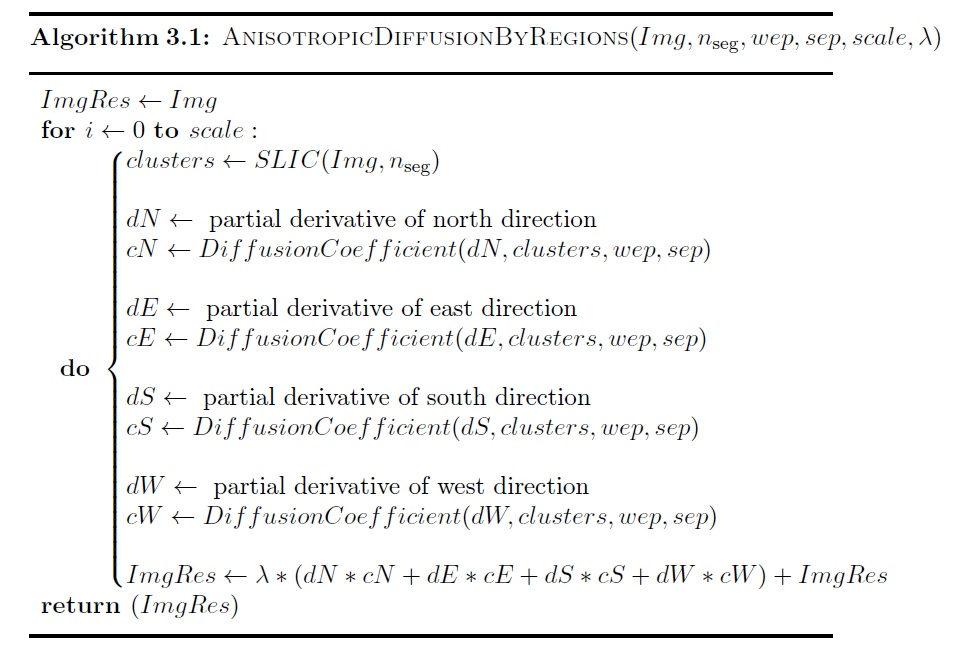
\includegraphics[width=8.3cm]{image/Alg1}
	\end{center}
	\caption{Algoritmo de Difusi\'on Anisotr\'opica por Regiones \label{fig:difusion_anisotropica_regiones}}
\end{figure}

La difusi\'on anisotr\'opica es el hilo principal del algoritmo, para llevarla a cabo dada una imagen inicial. Con el algoritmo de $SLIC$ se divide la imagen por regiones o segmentos, entonces se busca la magnitud del gradiante $||\nabla I||$ como las componentes direccionales mostradas el la secci\'on 1.2. La segmentaci\'on obtenida tambi\'en se asocia a cada imagen de degradado, por tanto, tambi\'en est\'an dividido por el mismo modelo que la imagen original.

\begin{figure}[htb]
	\begin{center}
		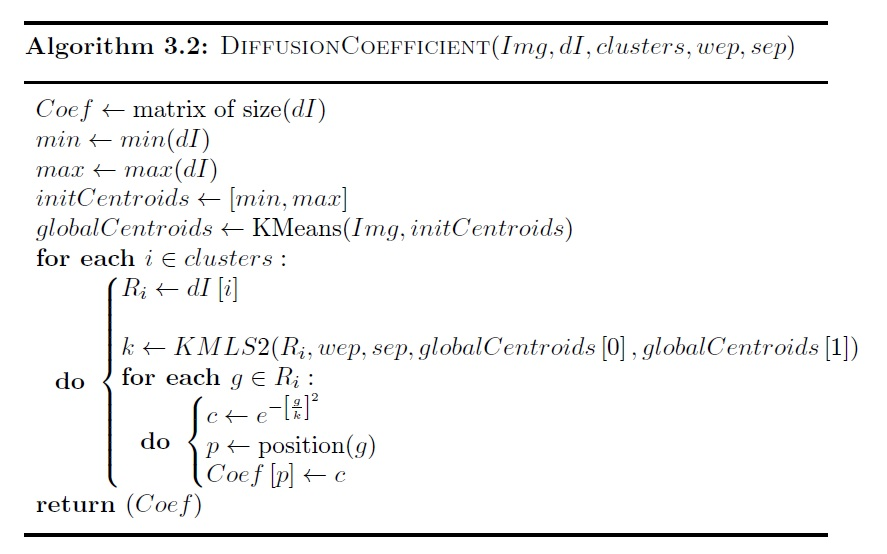
\includegraphics[width=8.3cm]{image/Alg2}
	\end{center}
	\caption{Algoritmo Coeficientes de Difusi\'on \label{fig:coeficientes_difusion}}
\end{figure}

Luego utilizamos el algorimto de estimaci\'on $KMMC2$ en cada segmento de las im\'agenes de degradado para obtener el par\'ametro de constraste $k$. Ya teniendo $k$ para una regi\'on, la matriz o imagen de coeficientes se construye por segmentos, donde cada p\'ixel de estos ser\'an calculados por (10) donde $||\nabla I(x,y,t)||$ es el valor que tiene la imagen del gradiente en esa posici\'on en el tiempo $t$ y el umbral $k$ asociado a esa regi\'on.

Solo resta efectuar la ecuaci\'on de difusi\'on anisotr\'opica dado que se poseen todas las derivadas y sus coeficientes. Como fue explicado la difusi\'on es un m\'etodo de espacio de escala, lo que significa que su funcionamiento y resultado depende de la cantidad de iteraciones del algoritmo. Para completarlo, a la imagen resultante se vuelve a procesar hasta completar las iteraciones establecidas.

\begin{figure}[htb]
	\begin{center}
		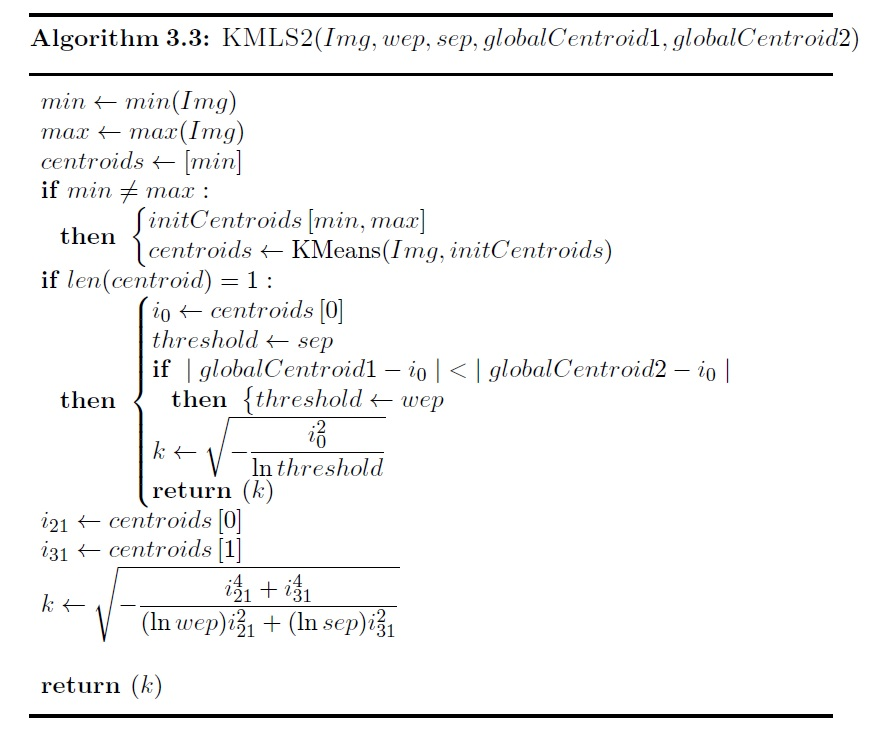
\includegraphics[width=8.3cm]{image/Alg3}
	\end{center}
	\caption{Algoritmo KMMC2 \label{fig:kmmc2}}
\end{figure}
%-----------------------------------------------------------------------------------

%-----------------------------------------------------------------------------------

\section{Experimentaci\'{o}n y resultados}\label{sec:experimentacion_resultados}

Este nuevo algoritmo propuesto por Richard Miguel M\'endez Castillo en 2019 \cite{richard} fue puesto a prueba como parte experimental con im\'agenes de mamograf\'ias, pues en este trabajo se propone dar continuidad a esta labor pero ahora con un nuevo tipo de im\'agenes, en este caso las im\'agenes de ultrasonidos. Estas im\'agenes fueron extra\'idas desde el motor de b\'usqueda de Google.

Incialmente se le aplicar\'a un filtro con un kernel gaussiano para la regularizaci\'on espacial, haciendo el proceso insensible al ruido. Esto evita la poca agilidad del algortimo AD-KMMC2 de malintepretar fuertes oscilaciones como bordes que necesitan ser mejorados. Los algoritmos se ejecutan inicialmente con los mismos par\'ametros de prueba que fueron utilizados en el caso de las mamograf\'ias, estos van a variar en n\'umero de iteracciones, cantidad de regiones para segmentar la imagen y umbrales de bordes. Se establecer\'a posible relaciones entre par\'ametros y resultados observados, sean \'estos visuales o de medidas de calidad.
%-----------------------------------------------------------------------------------
\subsection{Medidas de calidad}\label{sec:medidas_calidad}

Cunado realizamos el procesamiento de una imagen debemos evaluar el resultado obtenido, como por ejemplo, si se realiza alg\'un tipo de suavizado o eliminaci\'on de ruido se querr\'a saber cual es la mejor una vez realizado el filtrado. Con el fin de no solo buscar una evaluaci\'on basada en el  sistema de visi\'on humana existen ciertas medidas que prueban diferentes patrones de calidad en la imagen, y los resultados no siempre son perceptible ante el ojo humano, pero en general, esos resultados se usan con frecuencia en investigaciones \cite{ferrari}.

En este trabajo al igual que en los anteriores se utilizar\'an las siguientes medidas de calidad:

\begin{enumerate}
\item Root Mean Square Error $(RMSE)$ \cite{gupta}:

Este es utilizado para medir la diferencia entre valores precedidos por un estimador (imagen resultante) y los valores reales de las observaciones (imagen original). Representa la desviaci\'on estandar de esa diferencia. Sirve para evaluar la magnitud del error de la predicci\'on. Mientras mayor sea el valor, entonces tendremos peores resultados. La forma de calcularlo es la siguiente:

\begin{equation}
	MSE = \frac{1}{MN} \sum_{x=1}^M \sum_{y=1}^N [I(x,y) - \hat{I} (x,y)]^2
\end{equation}

\begin{equation}
	RMSE = \sqrt{MSE}
\end{equation}
donde $M$ y $N$ son las dimensiones de la imagen. En este caso es v\'alido resaltar que la resta mide que tan diferente es la imagen original a la resultante, por lo que mientras menor sea esta diferencia mayor parecido entre p\'ixel y p\'ixel se alcanza. En el caso particular que las im\'agenes sean iguales entonces $MSE = 0$.

\item Peak Signal-to-Noise Ration $(PSNR)$ \cite{perona_malik}:

Esta media se considera una aproximaci\'on de la presepci\'on visual humana de la calidad de la reconstrucci\'on. Representa entre el m\'aximo valor posible de una se\~nal(p\'ixel de imagen sin ruido) y el poder de corrupci\'on del ruido(imagen mejorada) que afecta la fidelidad de esta representaci\'on. Su valor es proporcional a la calidad del resultado, como consecuencia de la $MSE$, y es muy utilizado para probar los procesos de difusi\'on \cite{krishnan}. Mientras mayor sea el valor de $PSNR$ mejor es el resultado obtenido. Expresado en funci\'on de $MSE$ queda de la forma:

\begin{equation}
	PSNR = 10 \cdot \log{10}{\left (\frac{MAX_I^2}{MSE}\right )}
\end{equation}

\item Signal to Noise Ratio $(SNR)$ \cite{achanta}:

\begin{equation}
	SNR = \frac{\mu}{\sigma}
\end{equation}
donde $\mu$ es la media de la intensidad de los p\'ixeles de la imegen procesada y $\sigma$  es la desviaci\'on estandar de la imagen original. En este caso buscamos la que tenga menor valor.
\end{enumerate}

%-----------------------------------------------------------------------------------
\subsection{Experimentaci\'on}\label{sec:experimentacion}

Los algoritmos $AD-KMMC$ y $AD-KMMC2$ se han implementado utilizando el lenguaje de programaci\'on Python 3.6. El experimento se realizar\'a con un $\lambda = \frac{1}{4}$ y seguir\'a los siguientes pasos:

\begin{enumerate}
\item Se tomar\'a una imagen de ultrasonido y se le aplicar\'a un filtro gaussiano con $\sigma=1$.
\item Se le aplicar\'a $AD-KMMC$ a esa imagen filtrada, con par\'ametros variados.
\item A la misma imagen filtrada y fijando los mismos par\'ametros del paso 2, se le aplicar\'a el nuevo algoritmo $AD-KMMC2$ a la imagen original despu\'es de la segmentaci\'on con $SLIC$ pero haciendo el n\'umero de segmento un par\'ametro variable.
\item La imagen original y los resultados de los pasos 2 y 3 se procesan utilizando el detector de bordes Scharr.
\item Las im\'agenes de bordes obtenidas en el paso 4 a partir de los resultados de los pasos 2 y 3 son sometida en comparaci\'on con la imagen obtenida en 4 (imagen de borde de la original) usando las tres medidas de calidad.
\end{enumerate}

\begin{figure}
	\centering
	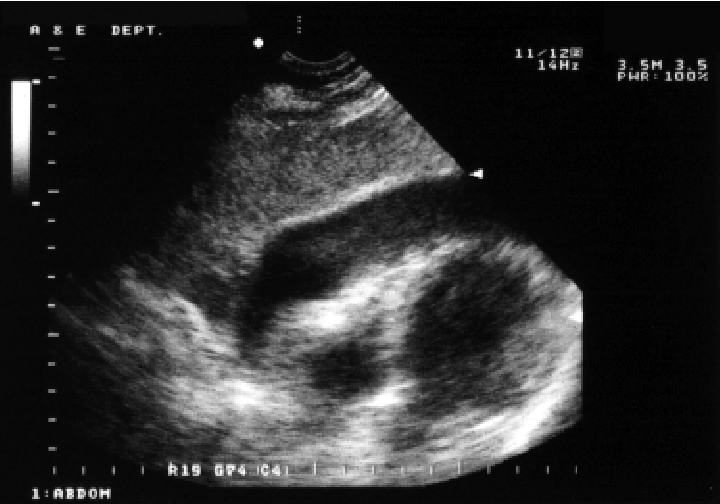
\includegraphics[width=4cm]{image/im1/im_1}
	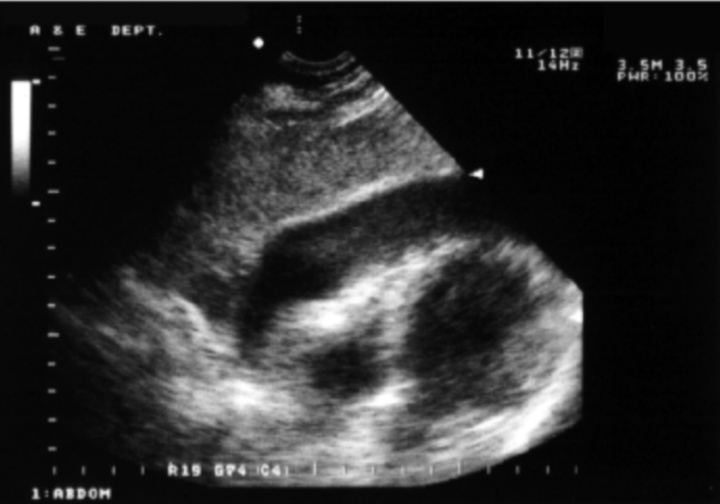
\includegraphics[width=4cm]{image/im1/im_1(mu=1)}
	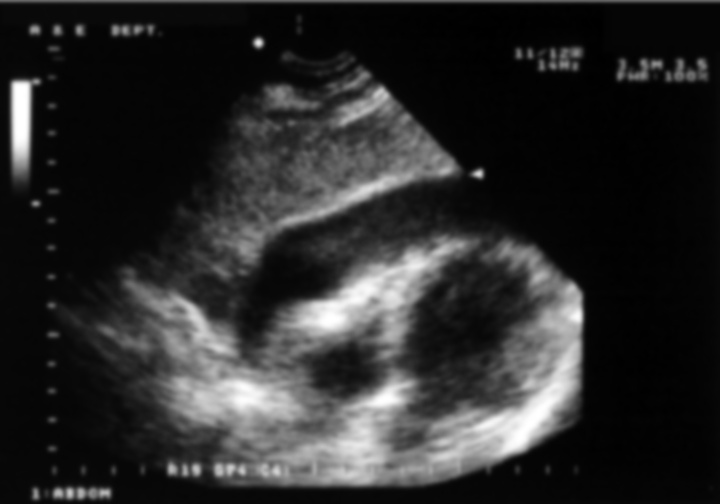
\includegraphics[width=4cm]{image/im1/im_1(mu=2)}
	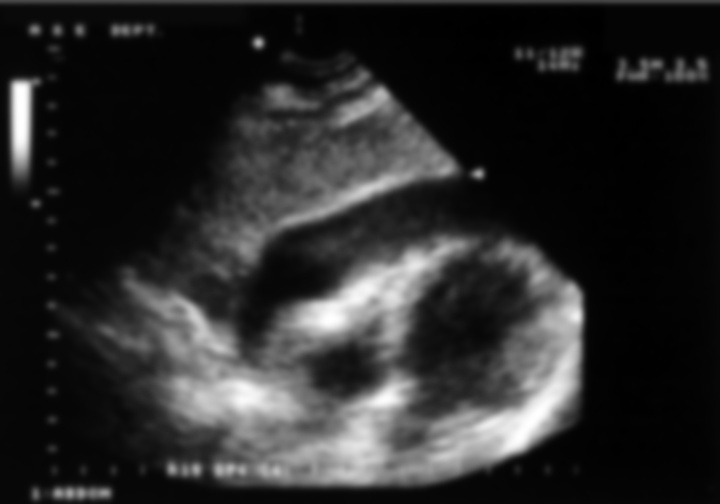
\includegraphics[width=4cm]{image/im1/im_1(mu=3)}
	\caption{Filtro gaussiano con $\sigma = 1, 2, 3$ \label{fig:filtro_gaussiano}}
\end{figure}

En el primer paso se menciona el hecho de aplicar un filtro gaussiano inicialmente a la imagen. Por este motivo se decidi\'o aplicar varios filtros gaussianos a las im\'agenes para comparar cual ser\'ia el m\'as apropiado a la hora de aplicar en este trabajo. A continuaci\'on se muestra los diferentes resultados obtenidos al aplicar dicho filtro con los valores $\sigma = 1,2,3$. En la figura \ref{fig:filtro_gaussiano} se muestra la imagen original y los respectivos resultados obtenidos de aplicar los filtros gaussianos.

Dado a simple vista, en lo que resta de este trabajo solo se usar\'a un filtro gaussiano con $\sigma = 1$, dado que un valor mayor implicar\'ia mayor borrosidad y p\'erdida de informaci\'on. Esto es consecuencia de la baja resoluci\'on de la imagen ya que de no ser as\'i, pudieramos usar valores mayores para $\sigma$.

%-----------------------------------------------------------------------------------
\subsection{Resultados}\label{sec:resultados}

A continuaci\'on se expondr\'a una serie de tablas y algunas im\'agenes resultantes del experimento realizado. Para esto, en cada tabla se tomar\'an un par  $(wep,\ sep)$ y en el caso que el nombre de la imagen est\'e acompa\~nado de un n\'umero entre par\'entesis estar\'a haciendo referencia al n\'umero de segmentos que se usar\'an en el algortimo de $SLIC$. 

Tambi\'en cabe destacar que en cada ejemplo se var\'ia el par\'ametro $t$, para poder comparar los resultados en cada iteraci\'on. Como l\'imite de iteraciones o tiempo de parada se tom\'o $t = 10$, pero esto no implica que no se puedan seleccionar valores mayores.

El expermiento se realiz\'o con un total de 10 im\'agenes de ultrasonido, de las cuales las 7 $(im_1\ -\ im_7)$ primeras fueron escogidas para exponer las medidas de calidad, 4 $(im_1, im_3,\ im_5,\ im_7)$ se muestran como ejemplo y 2 $(im_8,\  im_{10} )$ se usaron para mostrar los resultados obtenidos una vez aplicado el algortimo $SLIC$.


%-----------------------------------------------------------------------------------
\subsection{Discusi\'{o}n}\label{sec:discusion}

Inicialmente pasaremos a analizar el comportamiento de las tablas teniendo en cuenta los resultados obtenidos por los alogitmos de $KMMC2$ y $KMMC$. En la tabla \ref{fig:tabla1} se puede observar que el $RMSE$ y $SNR$ son menores para $KMMC2$ que en $KMMC$, pues cabe recordar que mientras menores sean estos valores mejor ser\'ian los resultados obtenidos. Pero en el caso de $PSNR$ pasa lo contrario, pues aqu\'i se busca obtener valores mayores, siendo en este caso mejor para $KMMC$, donde la menor diferencia es de 8 aproximadamente. A diferencia de la tabla \ref{fig:tabla1} que solo se realizaron 4 iteraciones en la tabla \ref{fig:tabla2} se realizan 10. En este caso todos los resultados obtenidos fueron mejor para el caso de $KMMC2$, y en algunos con diferencias muy notables. En estos casos tambi\'en hay que tener en cuenta que en cada imagen se tienen n\'umeros de segmentos diferentes.

Ya en la tabla \ref{fig:tabla3} se mantiene el mismo n\'umero de segmentos para as\'i, poder tener una mejor idea de lo que pasa. En este caso las diferencias en el $RMSE$ son notables y ahora de una manera m\'as uniforme para $KMMC2$ que en las tablas anterirores. A pesar que en $KMMC2$ los valores de $PSNR$ son mejores, este no var\'ia mucho, al igual que pasa con $SNR$.

En el caso de la tabla \ref{fig:tabla4} se mantienen todos los par\'ametros fijos y se analiza el comportamiento de dos im\'agenes desde la iteraci\'on 1 hasta la 10. En este caso se tom\'o la imagen de mejor resoluci\'on y la de peor. Para el caso de la imagen 1 se ve que las medidas $PSNR$ y $SNR$ se comportan de forma leve, pero con mejor\'ia, sin embargo, $RMSE$ no, inicialmente decrece, pero llega un punto en que se revierte.

En los ejemplos ilustrados en este trabajo se puede observar que las im\'agenes resaltan bien los bordes, pero a diferencia de las mamograf\'ias, los ultrasonidos poseen una mayor cantidad de bordes, por lo que el cambio brusco de intensidad en los p\'ixeles que ocurre es mucho mayor. En los ejemplos ilustrados se puede observar como los bordes son detectados, pero se nota un grosor borroso en ellos, a diferencia de trabajos antecesores que estos eran m\'as finos y precisos. Dado a las caracter\'isticas de este tipo de im\'agenes, donde predomina mucha variaci\'on de contraste, una vez aplicado el algoritmo, queda en las zonas centrales una especie de neblina, con \'areas m\'as intensas que otras.
  
%===================================================================================
% Conclusiones
%-----------------------------------------------------------------------------------
\section{Conclusiones}\label{sec:conclusiones}

Una vez probado el desempe\~no del algortimo propuesto por Richard Miguel M\'endez Castillo en 2019 en su trabajo referente a im\'agenes de mamograf\'ias, se decidi\'o extender para otro tipo de im\'agenes m\'edicas, en este caso, im\'agenes de ultrasonido. Se corrobor\'o que el nuevo algoritmo $KMMC2$ tiene un mejor rendimiento, ya que el procesamiento local, con la segmentación $SLIC$, es una herramienta importante para tratar con regiones homog\'eneas o de muy bajo contraste.

En algunos casos del experimento no se lleg\'o a los resultados esperados, ya que el $KMMC2$ tuvo un peor desepe\~no, pero por lo general y en los ejemplos visuales se pudo observar como el resultado obtenido en percepci\'on humana es notable. Tambi\'en hay que destacar que todos los experimentos tuvieron como l\'imite 10 iteraciones, pero esto no implica que este sea el mejor resultado, o un tiempo de parada \'optimo, incluso, se vi\'o como no siempre mientras mayor el n\'umero de iteracciones mejor el resultado.

A pesar de que fueron usadas algunas im\'agenes, estas no son suficientes como para dar un resultado final, por ende se recomienda utilizar otro tipos de im\'agenes, al igual que otras im\'agenes de ultrasonidos de mejor resoluci\'on, para as\'i ver el desempe\~no completo del algoritmo. Tambi\'en ser\'ia importante tener en cuenta que existen ultrasonidos de varias zonas del cuerpo humano, ser\'ia de gran utilidad poder procesar ejemplos de cada una, para as\'i tener, una idea m\'as general.

%===================================================================================
% Conclusiones
%-----------------------------------------------------------------------------------
\section{Anexos}\label{sec:anexos}

\begin{figure}[!htb]
	\centering
	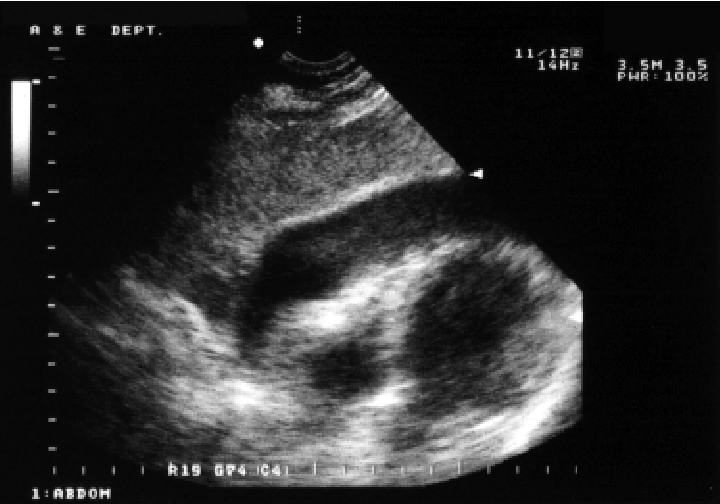
\includegraphics[width=3.8cm]{image/im1/im_1}
	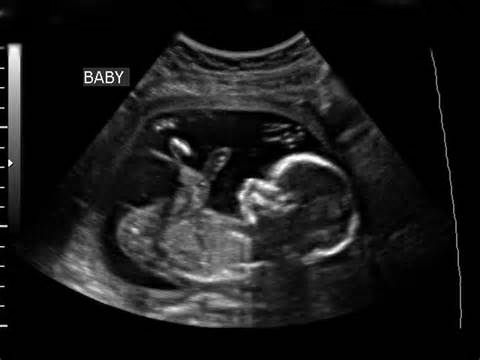
\includegraphics[width=3.8cm]{image/im3/im_3}
	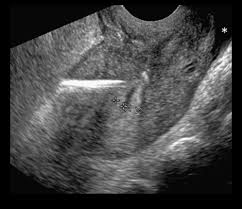
\includegraphics[width=3.8cm]{image/im5/im_5}
	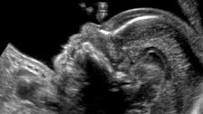
\includegraphics[width=3.8cm]{image/im7/im_7}
	\caption{Im\'agenes a analizar \label{fig:imagenes_analizar}}
\end{figure}

\begin{center}
	\begin{figure*}[!htb]
		\begin{subfigure}[a!]{4cm}
			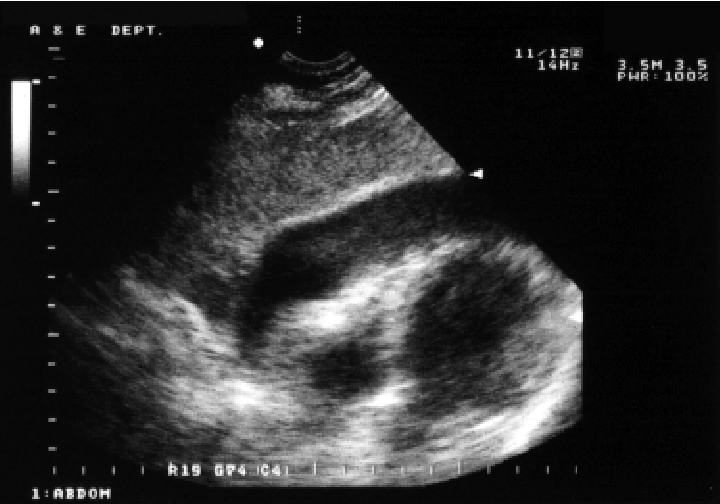
\includegraphics[width=4cm]{image/im1/im_1}
			\caption{Original}
		\end{subfigure}
		\begin{subfigure}[b!]{4cm}
			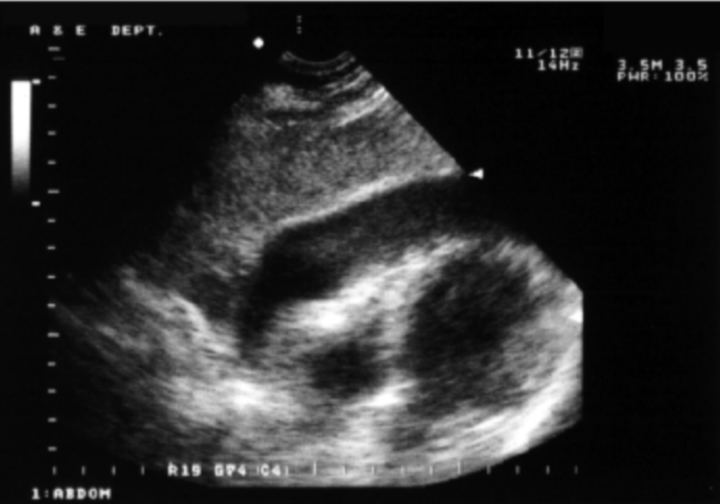
\includegraphics[width=4cm]{image/im1/im_1_noise}
			\caption{Filtered}
		\end{subfigure}
		\begin{subfigure}[c!]{4cm}
			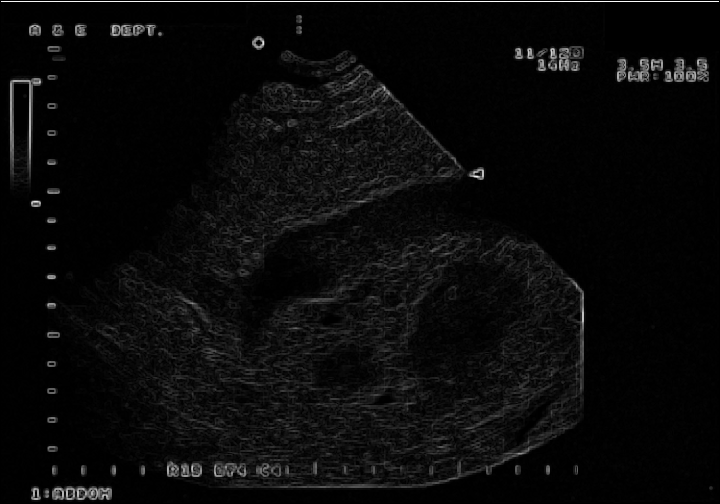
\includegraphics[width=4cm]{image/im1/im_1_edge}
			\caption{Edges}
		\end{subfigure}
		
		\begin{subfigure}[d!]{4cm}
			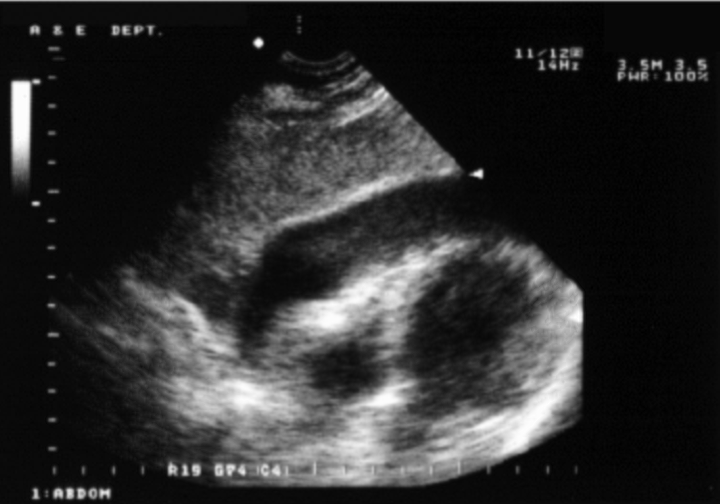
\includegraphics[width=4cm]{image/im1/im_1_4}
			\caption{KMMC2 $t = 4$}
		\end{subfigure}
		\begin{subfigure}[e!]{4cm}
			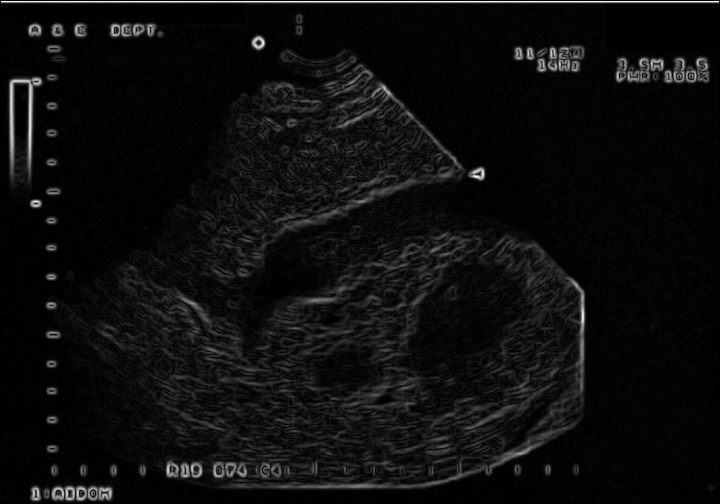
\includegraphics[width=4cm]{image/im1/im_1_4_edge}
			\caption{KMMC2 edge $t = 4$}
		\end{subfigure}
		\begin{subfigure}[f!]{4cm}
			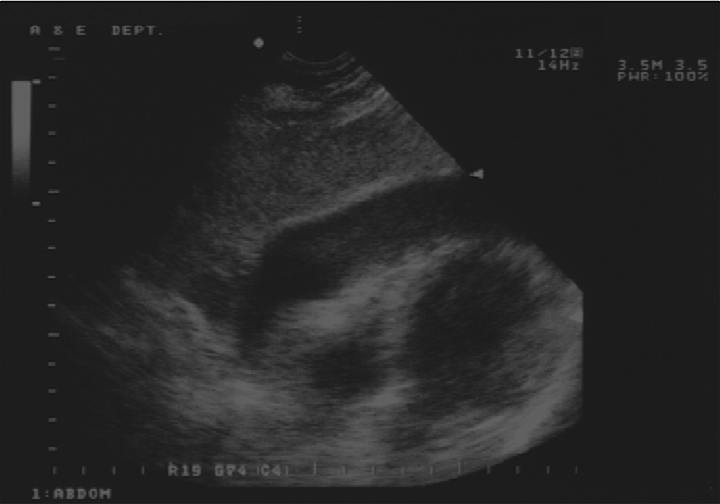
\includegraphics[width=4cm]{image/im1/im_1_4_norm}
			\caption{KMMC $t = 4$}
		\end{subfigure}
		\begin{subfigure}[g!]{4cm}
			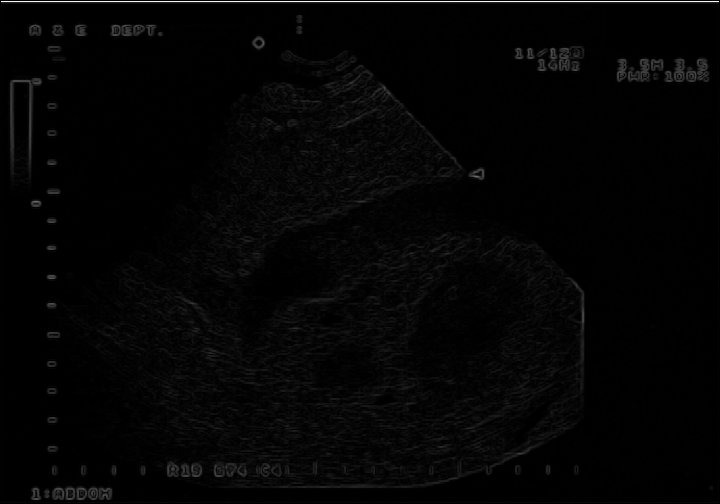
\includegraphics[width=4cm]{image/im1/im_1_4_norm_edge}
			\caption{KMMC edge $t = 4$}
		\end{subfigure}
		
		\begin{subfigure}[d!]{4cm}
			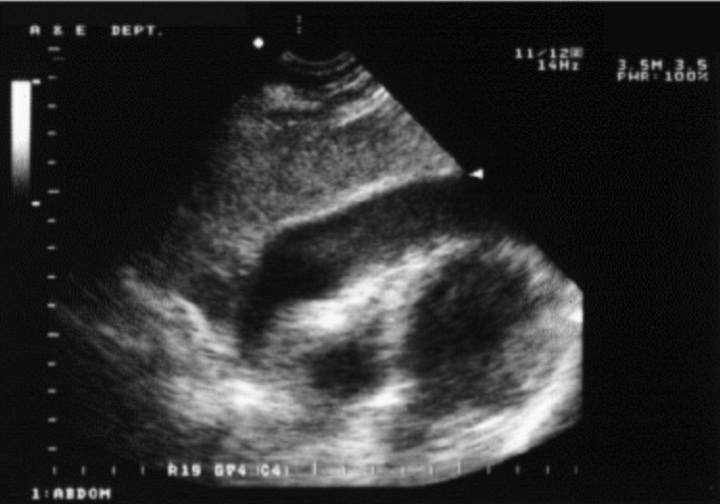
\includegraphics[width=4cm]{image/im1/im_1_10}
			\caption{KMMC2 $t = 10$}
		\end{subfigure}
		\begin{subfigure}[i!]{4cm}
			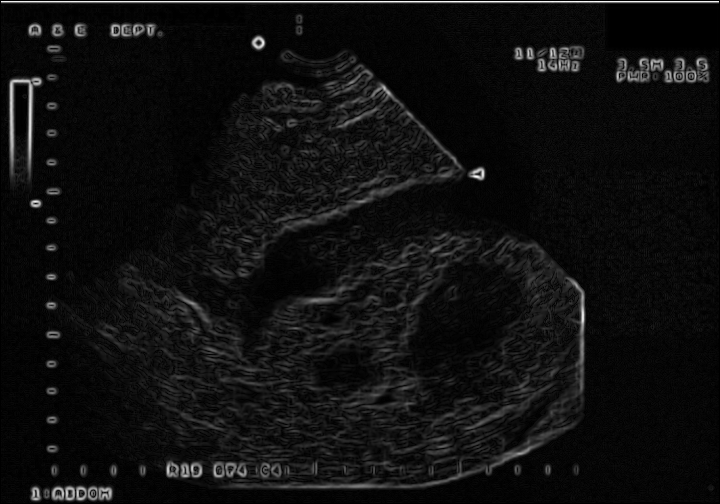
\includegraphics[width=4cm]{image/im1/im_1_10_edge}
			\caption{KMMC2 edge $t = 10$}
		\end{subfigure}
		\begin{subfigure}[j!]{4cm}
			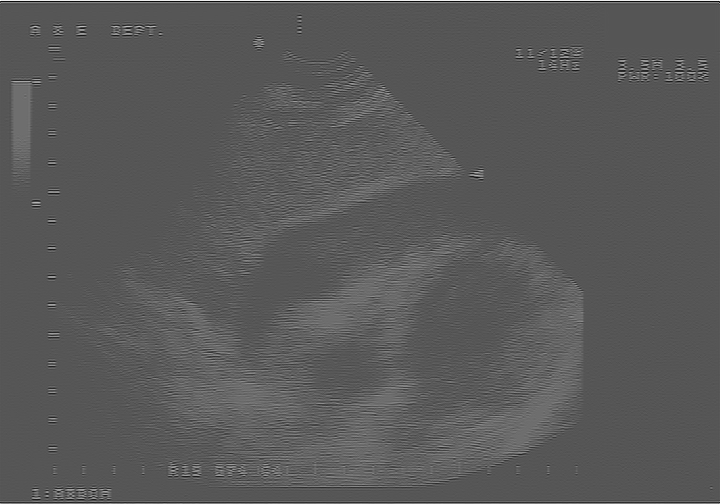
\includegraphics[width=4cm]{image/im1/im_1_10_norm}
			\caption{KMMC $t = 10$}
		\end{subfigure}
		\begin{subfigure}[k!]{4cm}
			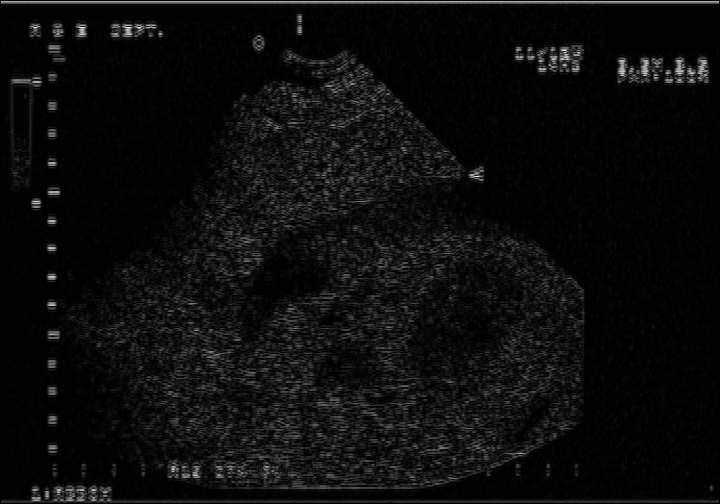
\includegraphics[width=4cm]{image/im1/im_1_10_norm_edge}
			\caption{KMMC edge $t = 10$}
		\end{subfigure}
		
		\caption{Im\_1 con par\'ametros $wep = 0.4590$, $sep = 0.0652$, $n = 14$}
	\end{figure*}
\end{center}

\begin{center}
	\begin{figure*}[!htb]
		\begin{subfigure}[a!]{4cm}
			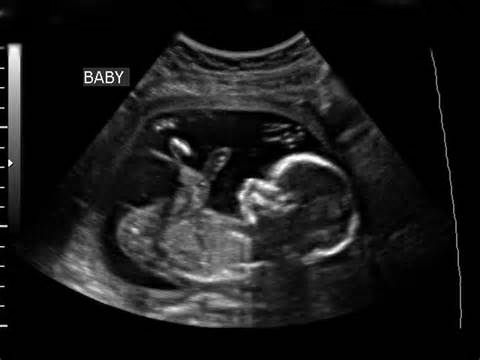
\includegraphics[width=4cm]{image/im3/im_3}
			\caption{Original}
		\end{subfigure}
		\begin{subfigure}[b!]{4cm}
			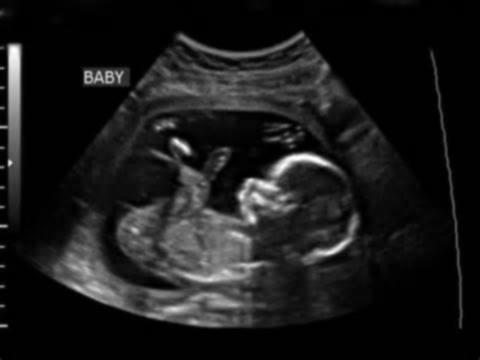
\includegraphics[width=4cm]{image/im3/im_3_noise}
			\caption{Filtered}
		\end{subfigure}
		\begin{subfigure}[c!]{4cm}
			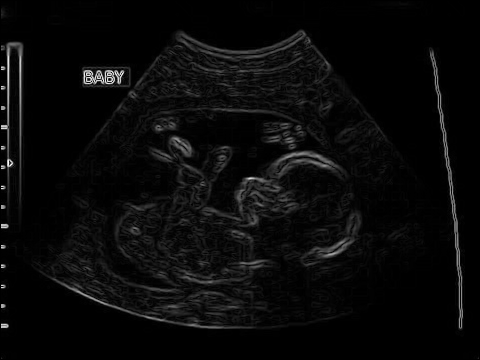
\includegraphics[width=4cm]{image/im3/im_3_edge}
			\caption{Edges}
		\end{subfigure}
		
		
		\begin{subfigure}[d!]{4cm}
			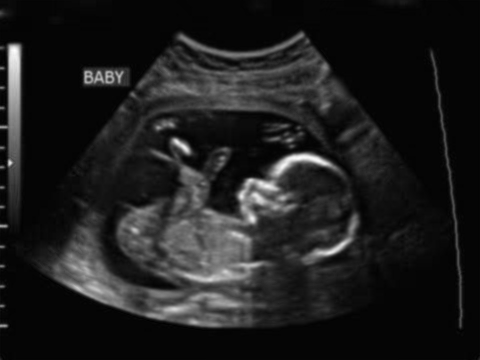
\includegraphics[width=4cm]{image/im3/im_3_4}
			\caption{KMMC2 $t = 4$}
		\end{subfigure}
		\begin{subfigure}[e!]{4cm}
			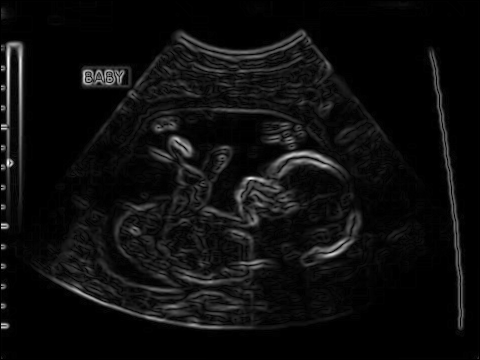
\includegraphics[width=4cm]{image/im3/im_3_4_edge}
			\caption{KMMC2 edge $t = 4$}
		\end{subfigure}
		\begin{subfigure}[f!]{4cm}
			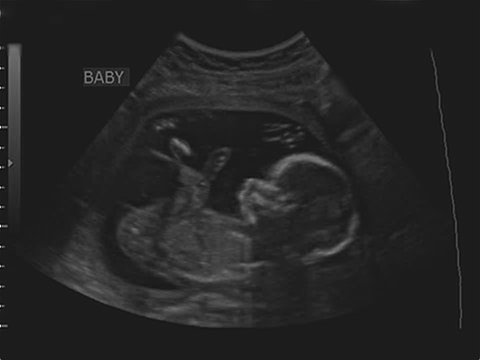
\includegraphics[width=4cm]{image/im3/im_3_4_norm}
			\caption{KMMC $t = 4$}
		\end{subfigure}
		\begin{subfigure}[g!]{4cm}
			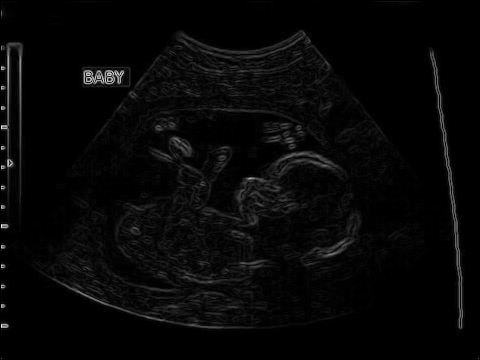
\includegraphics[width=4cm]{image/im3/im_3_4_norm_edge}
			\caption{KMMC edge $t = 4$}
		\end{subfigure}
		
		\begin{subfigure}[h!]{4cm}
			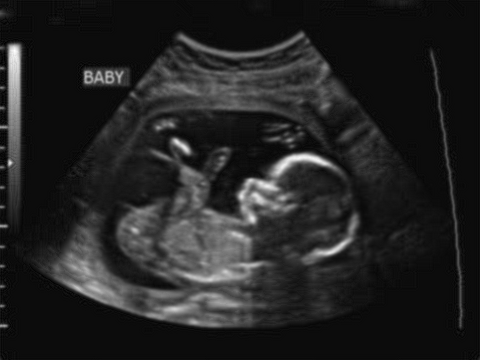
\includegraphics[width=4cm]{image/im3/im_3_10}
			\caption{KMMC2 $t = 10$}
		\end{subfigure}
		\begin{subfigure}[i!]{4cm}
			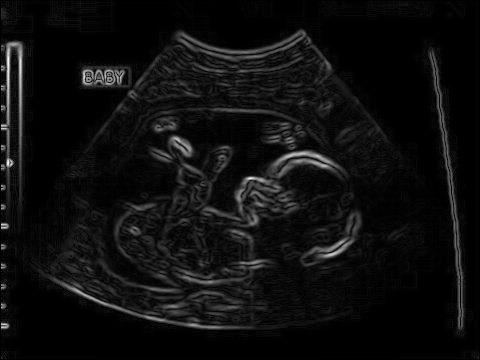
\includegraphics[width=4cm]{image/im3/im_3_10_edge}
			\caption{KMMC2 edge $t = 10$}
		\end{subfigure}
		\begin{subfigure}[j!]{4cm}
			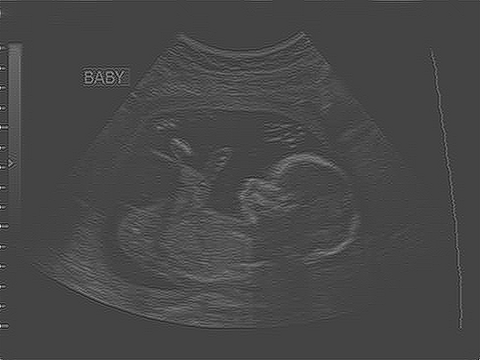
\includegraphics[width=4cm]{image/im3/im_3_10_norm}
			\caption{KMMC $t = 10$}
		\end{subfigure}
		\begin{subfigure}[k!]{4cm}
			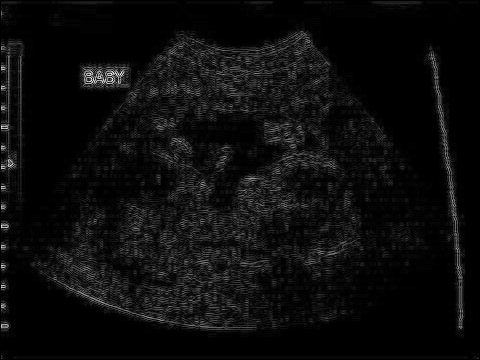
\includegraphics[width=4cm]{image/im3/im_3_10_norm_edge}
			\caption{KMMC edge $t = 10$}
		\end{subfigure}
		
		\caption{Im\_3 con par\'ametros $wep = 0.6614$, $sep = 0.0179$, $n = 23$}
	\end{figure*}
\end{center}

\newpage

\begin{center}
	\begin{figure*}[!htb]
		\begin{subfigure}[a!]{4cm}
			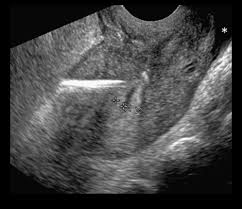
\includegraphics[width=4cm]{image/im5/im_5}
			\caption{Original}
		\end{subfigure}
		\begin{subfigure}[b!]{4cm}
			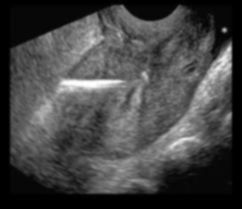
\includegraphics[width=4cm]{image/im5/im_5_noise}
			\caption{Filtered}
		\end{subfigure}
		\begin{subfigure}[c!]{4cm}
			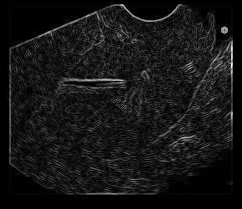
\includegraphics[width=4cm]{image/im5/im_5_edge}
			\caption{Edges}
		\end{subfigure}
		
		
		\begin{subfigure}[d!]{4cm}
			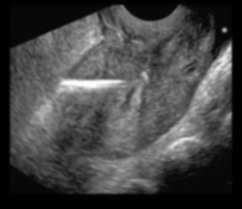
\includegraphics[width=4cm]{image/im5/im_5_4}
			\caption{KMMC2 $t = 4$}
		\end{subfigure}
		\begin{subfigure}[e!]{4cm}
			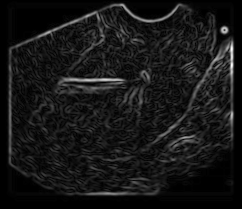
\includegraphics[width=4cm]{image/im5/im_5_4_edge}
			\caption{KMMC2 edge $t = 4$}
		\end{subfigure}
		\begin{subfigure}[f!]{4cm}
			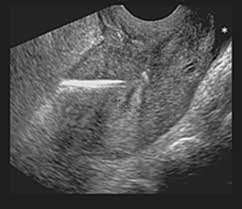
\includegraphics[width=4cm]{image/im5/im_5_4_norm}
			\caption{KMMC $t = 4$}
		\end{subfigure}
		\begin{subfigure}[g!]{4cm}
			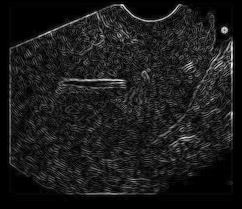
\includegraphics[width=4cm]{image/im5/im_5_4_norm_edge}
			\caption{KMMC edge $t = 4$}
		\end{subfigure}
		
		\begin{subfigure}[h!]{4cm}
			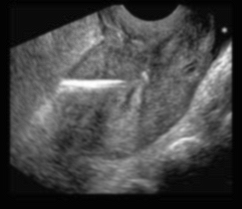
\includegraphics[width=4cm]{image/im5/im_5_10}
			\caption{KMMC2 $t = 10$}
		\end{subfigure}
		\begin{subfigure}[i!]{4cm}
			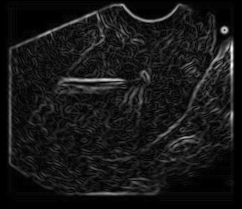
\includegraphics[width=4cm]{image/im5/im_5_10_edge}
			\caption{KMMC2 edge $t = 10$}
		\end{subfigure}
		\begin{subfigure}[j!]{4cm}
			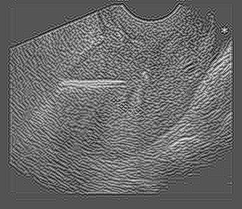
\includegraphics[width=4cm]{image/im5/im_5_10_norm}
			\caption{KMMC $t = 10$}
		\end{subfigure}
		\begin{subfigure}[k!]{4cm}
			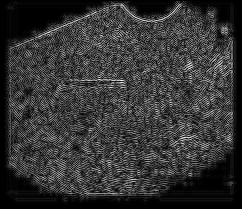
\includegraphics[width=4cm]{image/im5/im_5_10_norm_edge}
			\caption{KMMC edge $t = 10$}
		\end{subfigure}
		
		\caption{Im\_5 con par\'ametros $wep = 0.2593$, $sep = 0.0889$, $n = 9$}
	\end{figure*}
\end{center}

\begin{center}
	\begin{figure*}[!htb]
		\begin{subfigure}[a!]{4cm}
			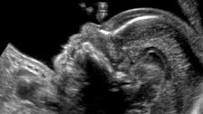
\includegraphics[width=4cm]{image/im7/im_7}
			\caption{Original}
		\end{subfigure}
		\begin{subfigure}[b!]{4cm}
			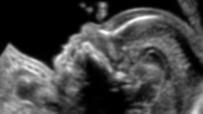
\includegraphics[width=4cm]{image/im7/im_7_noise}
			\caption{Filtered}
		\end{subfigure}
		\begin{subfigure}[c!]{4cm}
			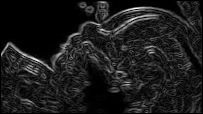
\includegraphics[width=4cm]{image/im7/im_7_edge}
			\caption{Edges}
		\end{subfigure}
		
		
		\begin{subfigure}[d!]{4cm}
			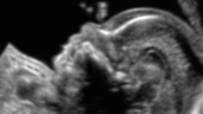
\includegraphics[width=4cm]{image/im7/im_7_4}
			\caption{KMMC2 $t = 4$}
		\end{subfigure}
		\begin{subfigure}[e!]{4cm}
			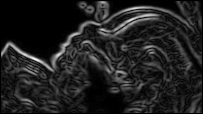
\includegraphics[width=4cm]{image/im7/im_7_4_edge}
			\caption{KMMC2 edge $t = 4$}
		\end{subfigure}
		\begin{subfigure}[f!]{4cm}
			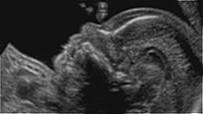
\includegraphics[width=4cm]{image/im7/im_7_4_norm}
			\caption{KMMC $t = 4$}
		\end{subfigure}
		\begin{subfigure}[g!]{4cm}
			\includegraphics[width=4cm]{image/im7/im_7_4_norm_edge}
			\caption{KMMC edge $t = 4$}
		\end{subfigure}
		
		\begin{subfigure}[h!]{4cm}
			\includegraphics[width=4cm]{image/im7/im_7_10}
			\caption{KMMC2 $t = 10$}
		\end{subfigure}
		\begin{subfigure}[i!]{4cm}
			\includegraphics[width=4cm]{image/im7/im_7_10_edge}
			\caption{KMMC2 edge $t = 10$}
		\end{subfigure}
		\begin{subfigure}[j!]{4cm}
			\includegraphics[width=4cm]{image/im7/im_7_10_norm}
			\caption{KMMC $t = 10$}
		\end{subfigure}
		\begin{subfigure}[k!]{4cm}
			\includegraphics[width=4cm]{image/im7/im_7_10_norm_edge}
			\caption{KMMC edge $t = 10$}
		\end{subfigure}
		
		\caption{Im\_7 con par\'ametros $wep = 0.5593$, $sep = 0.0652$, $n = 14$}
	\end{figure*}
\end{center}

\newpage

\begin{center}
	\begin{figure*}[!htb]
		\centering
		\includegraphics[width=5.5cm]{image/slic/im_8_color_14}
		\includegraphics[width=5.5cm]{image/slic/im_8_black_14}
		\includegraphics[width=5.5cm]{image/slic/im_8_white_14}
		\caption{Im\_8 $SLIC$ en Windows, $n = 14$}
	\end{figure*}
\end{center}

\begin{center}
	\begin{figure*}[!htb]
		\centering
		\includegraphics[width=5.5cm]{image/slic/im_10_color_23}
		\includegraphics[width=5.5cm]{image/slic/im_10_black_23}
		\includegraphics[width=5.5cm]{image/slic/im_10_white_23}
		\caption{Im\_10 $SLIC$ en Windows, $n = 23$}
	\end{figure*}
\end{center}

\begin{center}
	\begin{table*}[!htb]
		\centering
		\caption{Resultados con par\'ametros $wep = 0.1512$, $sep = 0.0351$, $t = 4$ \label{fig:tabla1}}
		\begin{tabular}{|c|c|c|c|c|c|c|}
			\hline
			Algoritmo & \multicolumn {3}{c |}{KMMC2} & \multicolumn {3}{c |}{KMMC} \\
			\hline
			Im\'agenes & RMSE & PSNR & SNR & RMSE & PSNR & SNR \\
			\hline
			im\_1(18) &  7.06110 & 23.61617 &  0.00065 & 13.28842 & 31.02648 & 0.00103 \\
			\hline
			im\_2(8) &  8.14287 & 20.22713 &  0.00157 & 5.92876 & 28.12158 & 0.00302 \\
			\hline
			im\_3(10) &  6.37224 & 24.22825 & 0.00095 & 5.07506 & 35.33467 & 0.00148 \\
			\hline
			im\_4(12) & 11.05530 & 20.34762 & 0.00105 & 17.17136 & 23.56271 & 0.00187 \\
			\hline
			im\_5(17) & 9.48456 & 19.85388 & 0.00255 & 7.12287 & 27.47691 & 0.00567 \\
			\hline
			im\_6(16) & 11.37647 & 19.98768 & 0.00132 & 8.63443 & 23.27591 & 0.00253 \\
			\hline
			im\_7(7) & 9.75062 & 19.39042 & 0.00425 & 8.97876 & 24.98165 & 0.00798 \\
			\hline
		\end{tabular}
	\end{table*}
\end{center}

\begin{center}
	\begin{table*}[!htb]
		\centering
		\caption{Resultados con par\'ametros $wep = 0.4590$, $sep = 0.0652$, $t = 10$ \label{fig:tabla2}}
		\begin{tabular}{|c|c|c|c|c|c|c|}
			\hline
			Algoritmo & \multicolumn {3}{c |}{KMMC2} & \multicolumn {3}{c |}{KMMC} \\
			\hline
			Im\'agenes & RMSE & PSNR & SNR & RMSE & PSNR & SNR \\
			\hline
			im\_1(16) & 7.19049 & 23.42316 & 0.00075 & 102.72220 & 21.40958 & 0.00706 \\
			\hline
			im\_2(16) & 8.12343 & 20.19310 & 0.00165 & 54.49810 & 12.41666 & 0.01106  \\
			\hline
			im\_3(9) & 6.56147 & 23.88787 & 0.00107 & 60.08620 & 22.26276 & 0.00664 \\
			\hline
			im\_4(8) & 11.24810 & 20.29872 & 0.00118 & 139.17860 & 17.80957 & 0.01245 \\
			\hline
			im\_5(18) & 9.40225 & 19.92589 & 0.00264 & 92.35204 & 12.80678 & 0.02629 \\
			\hline
			im\_6(16) & 11.36068 & 20.04932 & 0.00143 & 34.15934 & 15.38585 & 0.00771 \\
			\hline
			im\_7(18) & 9.78623 & 19.37734 & 0.00432 & 55.97011 & 12.34946 & 0.02204 \\
			\hline
		\end{tabular}
	\end{table*}
\end{center}

\begin{center}
	\begin{table*}[!htb]
		\centering
		\caption{Resultados con par\'ametros $wep = 0.6614$, $sep = 0.0179$, $t = 8$ \label{fig:tabla3}}
		\begin{tabular}{|c|c|c|c|c|c|c|}
			\hline
			Algoritmo & \multicolumn {3}{c |}{KMMC2} & \multicolumn {3}{c |}{KMMC} \\
			\hline
			Im\'agenes & RMSE & PSNR & SNR & RMSE & PSNR & SNR \\
			\hline
			im\_1(14) & 7.19902 & 23.44800 & 0.00074 & 42.04220 & 24.22972 & 0.00293 \\
			\hline
			im\_2(14) & 8.13200 & 20.16766 & 0.00161 & 36.10134 & 14.63316 & 0.00799 \\
			\hline
			im\_3(14) & 6.50122 & 23.95853 & 0.00103 & 32.84366 & 26.15773 & 0.00372 \\
			\hline
			im\_4(14) & 11.13977 & 20.32703 & 0.00112 & 59.80577 & 20.27990 & 0.00570 \\
			\hline
			im\_5(14) & 9.39104 & 19.90574 & 0.00263 & 72.03239 & 13.86125 & 0.02104 \\
			\hline
			im\_6(14) & 11.32550 & 20.05285 & 0.00144 & 24.75971 & 16.91503 & 0.00594 \\
			\hline
			im\_7(14) & 9.77511 & 19.43448 & 0.00429 & 37.35249 & 14.26154 & 0.01649 \\
			\hline
		\end{tabular}
	\end{table*}
\end{center}

\newpage

\begin{center}
	\begin{table*}[!htb]
		\centering
		\caption{KMMC2 con par\'ametros $wep = 0.5593$, $sep = 0.0652$ \label{fig:tabla4}}
		\begin{tabular}{|c|c|c|c|c|c|c|}
			\hline
			Im\'agenes & \multicolumn {3}{c |}{im\_1(14)} & \multicolumn {3}{c |}{im\_7(14)} \\
			\hline
			Iteraciones (t) & RMSE & PSNR & SNR & RMSE & PSNR & SNR \\
			\hline
			01 & 7.07037 & 23.60478 & 0.00062 & 9.79446 & 19.37714 & 0.00420 \\
			\hline
			02 & 7.05974 & 23.61785 & 0.00063 & 9.78304 & 19.39270 & 0.00421 \\
			\hline
			03 & 7.05350 & 23.62553 & 0.00065 & 9.77696 & 19.40306 & 0.00423 \\
			\hline
			04 & 7.05716 & 23.62101 & 0.00067 & 9.77302 & 19.41102 & 0.00424 \\
			\hline
			05 & 7.07714 & 23.59647 & 0.00069 & 9.76719 & 19.42007 & 0.00426 \\
			\hline
			06 & 7.11330 & 23.55219 & 0.00072 & 9.76526 & 19.42539 & 0.00428 \\
			\hline
			07 & 7.15461 & 23.50190 & 0.00074 & 9.76127 & 19.42610 & 0.00430 \\
			\hline
			08 & 7.19203 & 23.45658 & 0.00075 & 9.75939 & 19.42481 & 0.00432 \\
			\hline
			09 & 7.20862 & 23.43658 & 0.00076 & 9.75879 & 19.42239 & 0.00434 \\
			\hline
			10 & 7.22280 & 23.41951 & 0.00076 & 9.75939 & 19.41898 & 0.00436 \\
			\hline
		\end{tabular}
	\end{table*}
\end{center}

%===================================================================================
% Bibliografía
%-----------------------------------------------------------------------------------
\begin{thebibliography}{99}
%-----------------------------------------------------------------------------------
	\bibitem{achanta} Achanta, Radhakrishna, Appu Shaji, Kevin Smith, Aurelien Lucchi, Pascal Fua, Sabine Susstrunk. 2012. SLIC superpixels compared to state-of-theart superpixel methods. Pattern Analysis and Machine Intelligence, IEEE Transactions on. 34(11): 2274–2282.
	
	\bibitem{borroto} Borroto Fern\'andez M, Gonz\'alez Hidalgo M, Le\'on Mec\'ias A. 2014. New estimation method of the contrast parameter for the Perona-Malik difusion equation. Computer Methods in Biomechanics and Biomedical Engineering: Imaging \& Visualization.
	
	\bibitem{darshita} Darshita Jain. 2019. Superpixels and SLIC. http://darshita1405.medium.com/superpixel-and-slic-6b2d8a6e4f08.
	
	\bibitem{ferrari} Ferrari, Ricardo J. 2013. Off-line determination of the optimal number of iterations of the robust anisotropic diffusion filter applied to denoising of brain MR images.
	
	\bibitem{galic} Gali\'c I, Weickert J, Welk M, Bruhn A, Belyaev A, Seodel HP. 2008. Image Compression with Anisotropic Diffusion. J Math Imaging. 31: 255-269.
	
	\bibitem{gupta} Gupta, Rishu, Elamvazuthil I, Faye I, Vasant R, George J. 2014. Comparative Analysis of Anisotropic Diffusion and Non Local Means on Ultrasound Images.
	
	\bibitem{hidalgo} Hidalgo Gato E. 2015. Estimaci\'on del p\'ametro de contraste para el suavizado por Difusi\'on Anisotr\'opica aplicado por regiones.
	
	\bibitem{krishnan} Krishnan, Akshara P, Paul J S. 2014. Image enhancement in intensity projected multichannel MRI using spatially adaptive directional anisotropic difusion.
	
	\bibitem{kroon} Kroon D. 2009. Numerical Optimization of Kernel Based Image Derivatives. Short Paper University Twente.
	
	\bibitem{perona_malik} Perona P, Malik J. 1990. Scale-space and edge detection using anisotropic diffusion. IEEE Trans Pattern Anal Mach Intell. 12(7): .629–639.
	
	\bibitem{richard} M\'endez Castillo R M. 2019. Image smoothing by regions: a parallel version for mammography edges enhancement.
	
	\bibitem{mark} Mark S, Alberto S Aguada. 2020. [PDF] Feature Extraction and Image Processing for Cpmputer Vision. (4): 399-432
	
	\bibitem{tsiotsios} Tsiotsios C, Petrou M. 2013. On the choice of the parameters for anisotropic diffusion in image processing. Pattern Recogn. 46(5): 1369–1381.
%-----------------------------------------------------------------------------------
\end{thebibliography}

%-----------------------------------------------------------------------------------

\label{end}

\end{document}

%===================================================================================
